% Created by tikzDevice version 0.9 on 2016-01-12 22:38:45
% !TEX encoding = UTF-8 Unicode
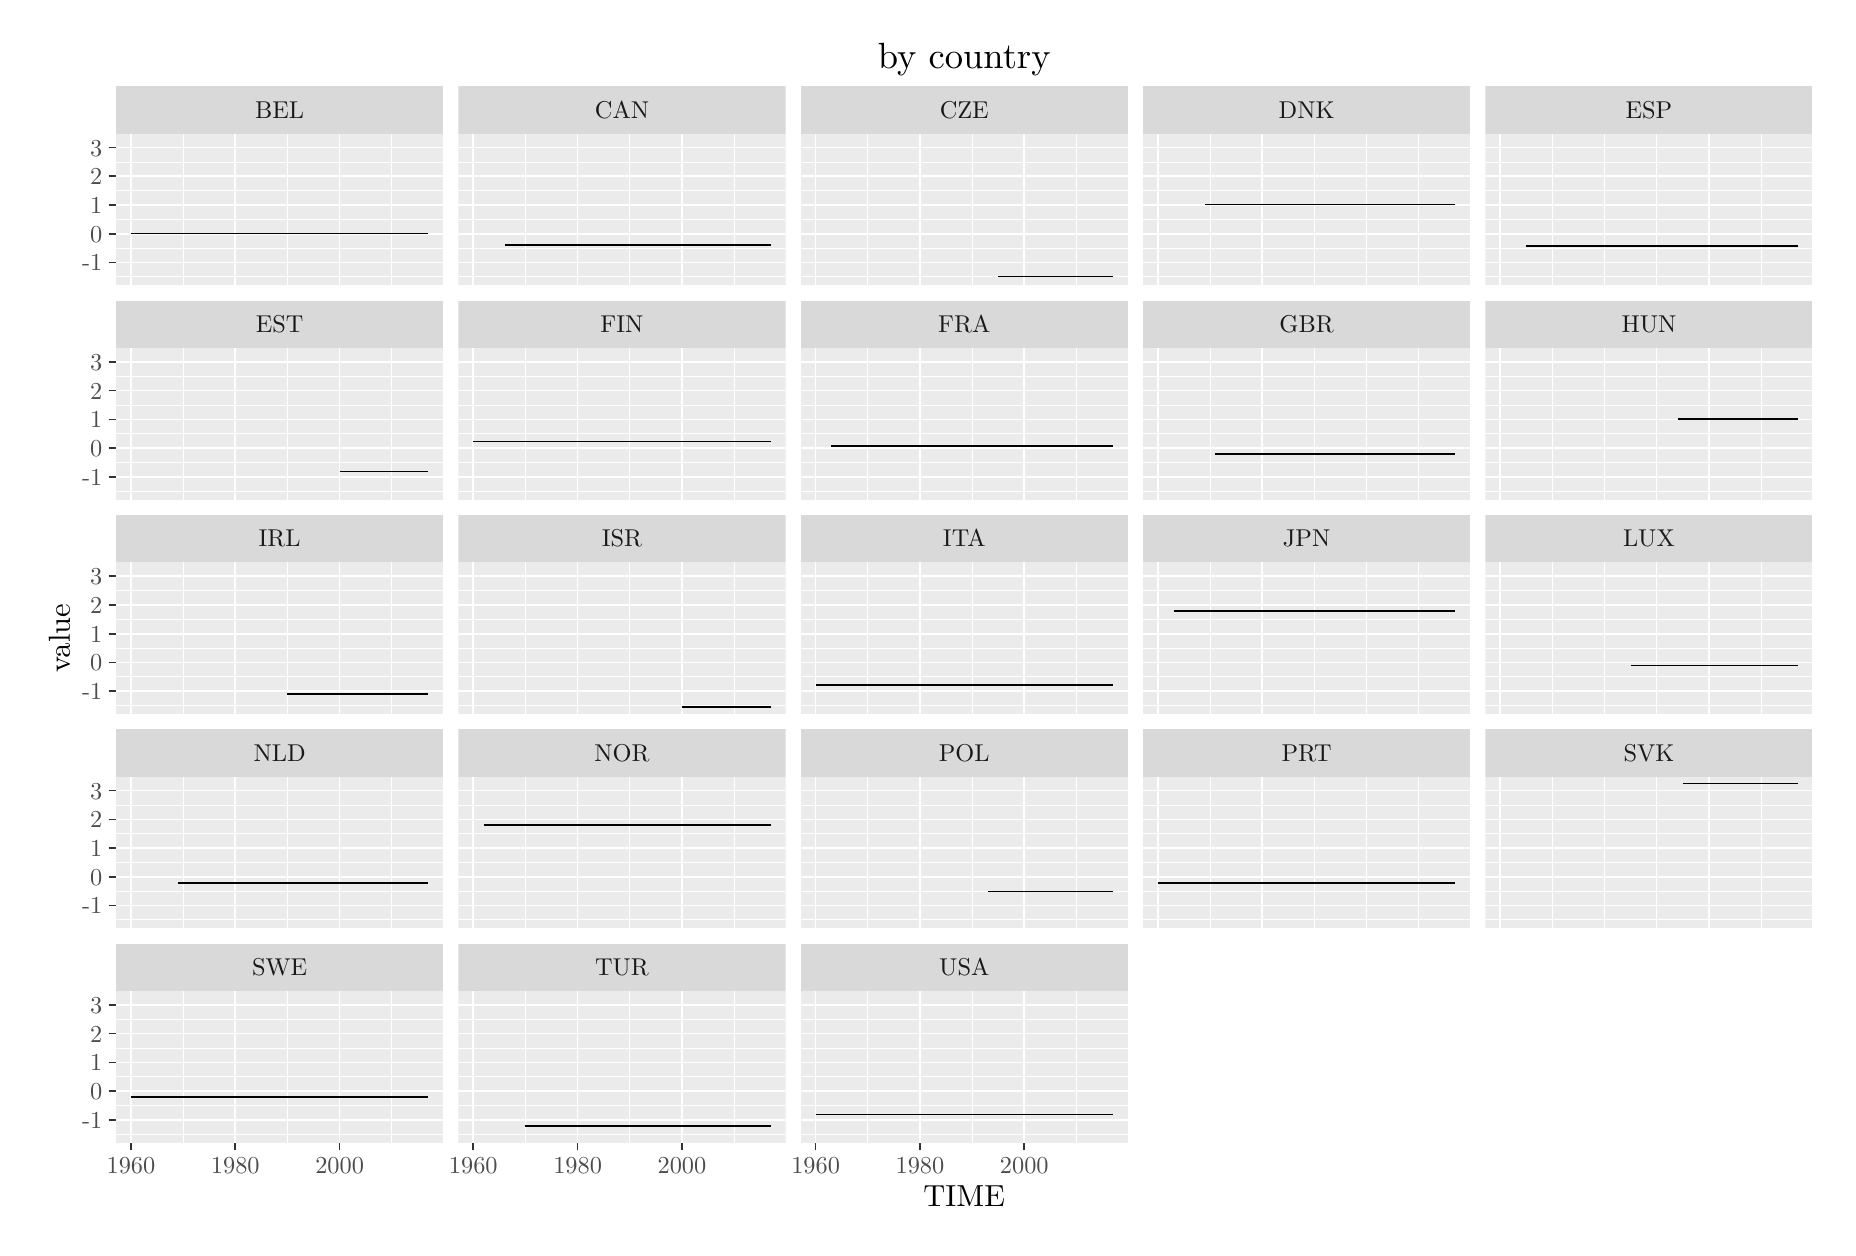
\begin{tikzpicture}[x=1pt,y=1pt]
\definecolor{fillColor}{RGB}{255,255,255}
\path[use as bounding box,fill=fillColor,fill opacity=0.00] (0,0) rectangle (650.43,433.62);
\begin{scope}
\path[clip] (  0.00,  0.00) rectangle (650.43,433.62);
\definecolor{drawColor}{RGB}{255,255,255}
\definecolor{fillColor}{RGB}{255,255,255}

\path[draw=drawColor,line width= 0.6pt,line join=round,line cap=round,fill=fillColor] (  0.00,  0.00) rectangle (650.43,433.62);
\end{scope}
\begin{scope}
\path[clip] ( 31.96,340.48) rectangle (150.15,395.37);
\definecolor{fillColor}{gray}{0.92}

\path[fill=fillColor] ( 31.96,340.48) rectangle (150.15,395.37);
\definecolor{drawColor}{RGB}{255,255,255}

\path[draw=drawColor,line width= 0.3pt,line join=round] ( 31.96,343.62) --
	(150.15,343.62);

\path[draw=drawColor,line width= 0.3pt,line join=round] ( 31.96,353.98) --
	(150.15,353.98);

\path[draw=drawColor,line width= 0.3pt,line join=round] ( 31.96,364.35) --
	(150.15,364.35);

\path[draw=drawColor,line width= 0.3pt,line join=round] ( 31.96,374.72) --
	(150.15,374.72);

\path[draw=drawColor,line width= 0.3pt,line join=round] ( 31.96,385.08) --
	(150.15,385.08);

\path[draw=drawColor,line width= 0.3pt,line join=round] ( 56.18,340.48) --
	( 56.18,395.37);

\path[draw=drawColor,line width= 0.3pt,line join=round] ( 93.88,340.48) --
	( 93.88,395.37);

\path[draw=drawColor,line width= 0.3pt,line join=round] (131.58,340.48) --
	(131.58,395.37);

\path[draw=drawColor,line width= 0.6pt,line join=round] ( 31.96,348.80) --
	(150.15,348.80);

\path[draw=drawColor,line width= 0.6pt,line join=round] ( 31.96,359.17) --
	(150.15,359.17);

\path[draw=drawColor,line width= 0.6pt,line join=round] ( 31.96,369.53) --
	(150.15,369.53);

\path[draw=drawColor,line width= 0.6pt,line join=round] ( 31.96,379.90) --
	(150.15,379.90);

\path[draw=drawColor,line width= 0.6pt,line join=round] ( 31.96,390.27) --
	(150.15,390.27);

\path[draw=drawColor,line width= 0.6pt,line join=round] ( 37.33,340.48) --
	( 37.33,395.37);

\path[draw=drawColor,line width= 0.6pt,line join=round] ( 75.03,340.48) --
	( 75.03,395.37);

\path[draw=drawColor,line width= 0.6pt,line join=round] (112.73,340.48) --
	(112.73,395.37);
\definecolor{drawColor}{RGB}{0,0,0}

\path[draw=drawColor,line width= 0.6pt,line join=round] ( 37.33,359.20) --
	( 39.22,359.20) --
	( 41.10,359.20) --
	( 42.99,359.20) --
	( 44.87,359.20) --
	( 46.76,359.20) --
	( 48.64,359.20) --
	( 50.53,359.20) --
	( 52.41,359.20) --
	( 54.30,359.20) --
	( 56.18,359.20) --
	( 58.07,359.20) --
	( 59.95,359.20) --
	( 61.84,359.20) --
	( 63.72,359.20) --
	( 65.61,359.20) --
	( 67.49,359.20) --
	( 69.38,359.20) --
	( 71.26,359.20) --
	( 73.15,359.20) --
	( 75.03,359.20) --
	( 76.92,359.20) --
	( 78.80,359.20) --
	( 80.69,359.20) --
	( 82.57,359.20) --
	( 84.46,359.20) --
	( 86.34,359.20) --
	( 88.23,359.20) --
	( 90.11,359.20) --
	( 92.00,359.20) --
	( 93.88,359.20) --
	( 95.77,359.20) --
	( 97.65,359.20) --
	( 99.54,359.20) --
	(101.42,359.20) --
	(103.31,359.20) --
	(105.19,359.20) --
	(107.08,359.20) --
	(108.96,359.20) --
	(110.85,359.20) --
	(112.73,359.20) --
	(114.62,359.20) --
	(116.50,359.20) --
	(118.39,359.20) --
	(120.27,359.20) --
	(122.16,359.20) --
	(124.04,359.20) --
	(125.93,359.20) --
	(127.81,359.20) --
	(129.70,359.20) --
	(131.58,359.20) --
	(133.47,359.20) --
	(135.35,359.20) --
	(137.24,359.20) --
	(139.12,359.20) --
	(141.01,359.20) --
	(142.89,359.20) --
	(144.78,359.20);
\end{scope}
\begin{scope}
\path[clip] (155.65,340.48) rectangle (273.85,395.37);
\definecolor{fillColor}{gray}{0.92}

\path[fill=fillColor] (155.65,340.48) rectangle (273.85,395.37);
\definecolor{drawColor}{RGB}{255,255,255}

\path[draw=drawColor,line width= 0.3pt,line join=round] (155.65,343.62) --
	(273.85,343.62);

\path[draw=drawColor,line width= 0.3pt,line join=round] (155.65,353.98) --
	(273.85,353.98);

\path[draw=drawColor,line width= 0.3pt,line join=round] (155.65,364.35) --
	(273.85,364.35);

\path[draw=drawColor,line width= 0.3pt,line join=round] (155.65,374.72) --
	(273.85,374.72);

\path[draw=drawColor,line width= 0.3pt,line join=round] (155.65,385.08) --
	(273.85,385.08);

\path[draw=drawColor,line width= 0.3pt,line join=round] (179.88,340.48) --
	(179.88,395.37);

\path[draw=drawColor,line width= 0.3pt,line join=round] (217.58,340.48) --
	(217.58,395.37);

\path[draw=drawColor,line width= 0.3pt,line join=round] (255.28,340.48) --
	(255.28,395.37);

\path[draw=drawColor,line width= 0.6pt,line join=round] (155.65,348.80) --
	(273.85,348.80);

\path[draw=drawColor,line width= 0.6pt,line join=round] (155.65,359.17) --
	(273.85,359.17);

\path[draw=drawColor,line width= 0.6pt,line join=round] (155.65,369.53) --
	(273.85,369.53);

\path[draw=drawColor,line width= 0.6pt,line join=round] (155.65,379.90) --
	(273.85,379.90);

\path[draw=drawColor,line width= 0.6pt,line join=round] (155.65,390.27) --
	(273.85,390.27);

\path[draw=drawColor,line width= 0.6pt,line join=round] (161.02,340.48) --
	(161.02,395.37);

\path[draw=drawColor,line width= 0.6pt,line join=round] (198.73,340.48) --
	(198.73,395.37);

\path[draw=drawColor,line width= 0.6pt,line join=round] (236.43,340.48) --
	(236.43,395.37);
\definecolor{drawColor}{RGB}{0,0,0}

\path[draw=drawColor,line width= 0.6pt,line join=round] (172.33,354.99) --
	(174.22,354.99) --
	(176.11,354.99) --
	(177.99,354.99) --
	(179.88,354.99) --
	(181.76,354.99) --
	(183.65,354.99) --
	(185.53,354.99) --
	(187.42,354.99) --
	(189.30,354.99) --
	(191.19,354.99) --
	(193.07,354.99) --
	(194.96,354.99) --
	(196.84,354.99) --
	(198.73,354.99) --
	(200.61,354.99) --
	(202.50,354.99) --
	(204.38,354.99) --
	(206.27,354.99) --
	(208.15,354.99) --
	(210.04,354.99) --
	(211.92,354.99) --
	(213.81,354.99) --
	(215.69,354.99) --
	(217.58,354.99) --
	(219.46,354.99) --
	(221.35,354.99) --
	(223.23,354.99) --
	(225.12,354.99) --
	(227.00,354.99) --
	(228.89,354.99) --
	(230.77,354.99) --
	(232.66,354.99) --
	(234.54,354.99) --
	(236.43,354.99) --
	(238.31,354.99) --
	(240.20,354.99) --
	(242.08,354.99) --
	(243.97,354.99) --
	(245.85,354.99) --
	(247.74,354.99) --
	(249.62,354.99) --
	(251.51,354.99) --
	(253.39,354.99) --
	(255.28,354.99) --
	(257.16,354.99) --
	(259.05,354.99) --
	(260.93,354.99) --
	(262.82,354.99) --
	(264.70,354.99) --
	(266.59,354.99) --
	(268.47,354.99);
\end{scope}
\begin{scope}
\path[clip] (279.35,340.48) rectangle (397.54,395.37);
\definecolor{fillColor}{gray}{0.92}

\path[fill=fillColor] (279.35,340.48) rectangle (397.54,395.37);
\definecolor{drawColor}{RGB}{255,255,255}

\path[draw=drawColor,line width= 0.3pt,line join=round] (279.35,343.62) --
	(397.54,343.62);

\path[draw=drawColor,line width= 0.3pt,line join=round] (279.35,353.98) --
	(397.54,353.98);

\path[draw=drawColor,line width= 0.3pt,line join=round] (279.35,364.35) --
	(397.54,364.35);

\path[draw=drawColor,line width= 0.3pt,line join=round] (279.35,374.72) --
	(397.54,374.72);

\path[draw=drawColor,line width= 0.3pt,line join=round] (279.35,385.08) --
	(397.54,385.08);

\path[draw=drawColor,line width= 0.3pt,line join=round] (303.57,340.48) --
	(303.57,395.37);

\path[draw=drawColor,line width= 0.3pt,line join=round] (341.27,340.48) --
	(341.27,395.37);

\path[draw=drawColor,line width= 0.3pt,line join=round] (378.97,340.48) --
	(378.97,395.37);

\path[draw=drawColor,line width= 0.6pt,line join=round] (279.35,348.80) --
	(397.54,348.80);

\path[draw=drawColor,line width= 0.6pt,line join=round] (279.35,359.17) --
	(397.54,359.17);

\path[draw=drawColor,line width= 0.6pt,line join=round] (279.35,369.53) --
	(397.54,369.53);

\path[draw=drawColor,line width= 0.6pt,line join=round] (279.35,379.90) --
	(397.54,379.90);

\path[draw=drawColor,line width= 0.6pt,line join=round] (279.35,390.27) --
	(397.54,390.27);

\path[draw=drawColor,line width= 0.6pt,line join=round] (284.72,340.48) --
	(284.72,395.37);

\path[draw=drawColor,line width= 0.6pt,line join=round] (322.42,340.48) --
	(322.42,395.37);

\path[draw=drawColor,line width= 0.6pt,line join=round] (360.12,340.48) --
	(360.12,395.37);
\definecolor{drawColor}{RGB}{0,0,0}

\path[draw=drawColor,line width= 0.6pt,line join=round] (350.70,343.74) --
	(352.58,343.74) --
	(354.47,343.74) --
	(356.35,343.74) --
	(358.24,343.74) --
	(360.12,343.74) --
	(362.01,343.74) --
	(363.89,343.74) --
	(365.78,343.74) --
	(367.66,343.74) --
	(369.55,343.74) --
	(371.43,343.74) --
	(373.32,343.74) --
	(375.20,343.74) --
	(377.09,343.74) --
	(378.97,343.74) --
	(380.86,343.74) --
	(382.74,343.74) --
	(384.63,343.74) --
	(386.51,343.74) --
	(388.40,343.74) --
	(390.28,343.74) --
	(392.17,343.74);
\end{scope}
\begin{scope}
\path[clip] (403.04,340.48) rectangle (521.24,395.37);
\definecolor{fillColor}{gray}{0.92}

\path[fill=fillColor] (403.04,340.48) rectangle (521.24,395.37);
\definecolor{drawColor}{RGB}{255,255,255}

\path[draw=drawColor,line width= 0.3pt,line join=round] (403.04,343.62) --
	(521.24,343.62);

\path[draw=drawColor,line width= 0.3pt,line join=round] (403.04,353.98) --
	(521.24,353.98);

\path[draw=drawColor,line width= 0.3pt,line join=round] (403.04,364.35) --
	(521.24,364.35);

\path[draw=drawColor,line width= 0.3pt,line join=round] (403.04,374.72) --
	(521.24,374.72);

\path[draw=drawColor,line width= 0.3pt,line join=round] (403.04,385.08) --
	(521.24,385.08);

\path[draw=drawColor,line width= 0.3pt,line join=round] (427.26,340.48) --
	(427.26,395.37);

\path[draw=drawColor,line width= 0.3pt,line join=round] (464.97,340.48) --
	(464.97,395.37);

\path[draw=drawColor,line width= 0.3pt,line join=round] (502.67,340.48) --
	(502.67,395.37);

\path[draw=drawColor,line width= 0.6pt,line join=round] (403.04,348.80) --
	(521.24,348.80);

\path[draw=drawColor,line width= 0.6pt,line join=round] (403.04,359.17) --
	(521.24,359.17);

\path[draw=drawColor,line width= 0.6pt,line join=round] (403.04,369.53) --
	(521.24,369.53);

\path[draw=drawColor,line width= 0.6pt,line join=round] (403.04,379.90) --
	(521.24,379.90);

\path[draw=drawColor,line width= 0.6pt,line join=round] (403.04,390.27) --
	(521.24,390.27);

\path[draw=drawColor,line width= 0.6pt,line join=round] (408.41,340.48) --
	(408.41,395.37);

\path[draw=drawColor,line width= 0.6pt,line join=round] (446.12,340.48) --
	(446.12,395.37);

\path[draw=drawColor,line width= 0.6pt,line join=round] (483.82,340.48) --
	(483.82,395.37);
\definecolor{drawColor}{RGB}{0,0,0}

\path[draw=drawColor,line width= 0.6pt,line join=round] (425.38,369.68) --
	(427.26,369.68) --
	(429.15,369.68) --
	(431.03,369.68) --
	(432.92,369.68) --
	(434.80,369.68) --
	(436.69,369.68) --
	(438.57,369.68) --
	(440.46,369.68) --
	(442.34,369.68) --
	(444.23,369.68) --
	(446.12,369.68) --
	(448.00,369.68) --
	(449.89,369.68) --
	(451.77,369.68) --
	(453.66,369.68) --
	(455.54,369.68) --
	(457.43,369.68) --
	(459.31,369.68) --
	(461.20,369.68) --
	(463.08,369.68) --
	(464.97,369.68) --
	(466.85,369.68) --
	(468.74,369.68) --
	(470.62,369.68) --
	(472.51,369.68) --
	(474.39,369.68) --
	(476.28,369.68) --
	(478.16,369.68) --
	(480.05,369.68) --
	(481.93,369.68) --
	(483.82,369.68) --
	(485.70,369.68) --
	(487.59,369.68) --
	(489.47,369.68) --
	(491.36,369.68) --
	(493.24,369.68) --
	(495.13,369.68) --
	(497.01,369.68) --
	(498.90,369.68) --
	(500.78,369.68) --
	(502.67,369.68) --
	(504.55,369.68) --
	(506.44,369.68) --
	(508.32,369.68) --
	(510.21,369.68) --
	(512.09,369.68) --
	(513.98,369.68) --
	(515.86,369.68);
\end{scope}
\begin{scope}
\path[clip] (526.74,340.48) rectangle (644.93,395.37);
\definecolor{fillColor}{gray}{0.92}

\path[fill=fillColor] (526.74,340.48) rectangle (644.93,395.37);
\definecolor{drawColor}{RGB}{255,255,255}

\path[draw=drawColor,line width= 0.3pt,line join=round] (526.74,343.62) --
	(644.93,343.62);

\path[draw=drawColor,line width= 0.3pt,line join=round] (526.74,353.98) --
	(644.93,353.98);

\path[draw=drawColor,line width= 0.3pt,line join=round] (526.74,364.35) --
	(644.93,364.35);

\path[draw=drawColor,line width= 0.3pt,line join=round] (526.74,374.72) --
	(644.93,374.72);

\path[draw=drawColor,line width= 0.3pt,line join=round] (526.74,385.08) --
	(644.93,385.08);

\path[draw=drawColor,line width= 0.3pt,line join=round] (550.96,340.48) --
	(550.96,395.37);

\path[draw=drawColor,line width= 0.3pt,line join=round] (588.66,340.48) --
	(588.66,395.37);

\path[draw=drawColor,line width= 0.3pt,line join=round] (626.36,340.48) --
	(626.36,395.37);

\path[draw=drawColor,line width= 0.6pt,line join=round] (526.74,348.80) --
	(644.93,348.80);

\path[draw=drawColor,line width= 0.6pt,line join=round] (526.74,359.17) --
	(644.93,359.17);

\path[draw=drawColor,line width= 0.6pt,line join=round] (526.74,369.53) --
	(644.93,369.53);

\path[draw=drawColor,line width= 0.6pt,line join=round] (526.74,379.90) --
	(644.93,379.90);

\path[draw=drawColor,line width= 0.6pt,line join=round] (526.74,390.27) --
	(644.93,390.27);

\path[draw=drawColor,line width= 0.6pt,line join=round] (532.11,340.48) --
	(532.11,395.37);

\path[draw=drawColor,line width= 0.6pt,line join=round] (569.81,340.48) --
	(569.81,395.37);

\path[draw=drawColor,line width= 0.6pt,line join=round] (607.51,340.48) --
	(607.51,395.37);
\definecolor{drawColor}{RGB}{0,0,0}

\path[draw=drawColor,line width= 0.6pt,line join=round] (541.53,354.61) --
	(543.42,354.61) --
	(545.30,354.61) --
	(547.19,354.61) --
	(549.07,354.61) --
	(550.96,354.61) --
	(552.84,354.61) --
	(554.73,354.61) --
	(556.61,354.61) --
	(558.50,354.61) --
	(560.38,354.61) --
	(562.27,354.61) --
	(564.15,354.61) --
	(566.04,354.61) --
	(567.92,354.61) --
	(569.81,354.61) --
	(571.69,354.61) --
	(573.58,354.61) --
	(575.46,354.61) --
	(577.35,354.61) --
	(579.23,354.61) --
	(581.12,354.61) --
	(583.01,354.61) --
	(584.89,354.61) --
	(586.78,354.61) --
	(588.66,354.61) --
	(590.55,354.61) --
	(592.43,354.61) --
	(594.32,354.61) --
	(596.20,354.61) --
	(598.09,354.61) --
	(599.97,354.61) --
	(601.86,354.61) --
	(603.74,354.61) --
	(605.63,354.61) --
	(607.51,354.61) --
	(609.40,354.61) --
	(611.28,354.61) --
	(613.17,354.61) --
	(615.05,354.61) --
	(616.94,354.61) --
	(618.82,354.61) --
	(620.71,354.61) --
	(622.59,354.61) --
	(624.48,354.61) --
	(626.36,354.61) --
	(628.25,354.61) --
	(630.13,354.61) --
	(632.02,354.61) --
	(633.90,354.61) --
	(635.79,354.61) --
	(637.67,354.61) --
	(639.56,354.61);
\end{scope}
\begin{scope}
\path[clip] ( 31.96,263.03) rectangle (150.15,317.92);
\definecolor{fillColor}{gray}{0.92}

\path[fill=fillColor] ( 31.96,263.03) rectangle (150.15,317.92);
\definecolor{drawColor}{RGB}{255,255,255}

\path[draw=drawColor,line width= 0.3pt,line join=round] ( 31.96,266.17) --
	(150.15,266.17);

\path[draw=drawColor,line width= 0.3pt,line join=round] ( 31.96,276.53) --
	(150.15,276.53);

\path[draw=drawColor,line width= 0.3pt,line join=round] ( 31.96,286.90) --
	(150.15,286.90);

\path[draw=drawColor,line width= 0.3pt,line join=round] ( 31.96,297.27) --
	(150.15,297.27);

\path[draw=drawColor,line width= 0.3pt,line join=round] ( 31.96,307.63) --
	(150.15,307.63);

\path[draw=drawColor,line width= 0.3pt,line join=round] ( 56.18,263.03) --
	( 56.18,317.92);

\path[draw=drawColor,line width= 0.3pt,line join=round] ( 93.88,263.03) --
	( 93.88,317.92);

\path[draw=drawColor,line width= 0.3pt,line join=round] (131.58,263.03) --
	(131.58,317.92);

\path[draw=drawColor,line width= 0.6pt,line join=round] ( 31.96,271.35) --
	(150.15,271.35);

\path[draw=drawColor,line width= 0.6pt,line join=round] ( 31.96,281.72) --
	(150.15,281.72);

\path[draw=drawColor,line width= 0.6pt,line join=round] ( 31.96,292.08) --
	(150.15,292.08);

\path[draw=drawColor,line width= 0.6pt,line join=round] ( 31.96,302.45) --
	(150.15,302.45);

\path[draw=drawColor,line width= 0.6pt,line join=round] ( 31.96,312.82) --
	(150.15,312.82);

\path[draw=drawColor,line width= 0.6pt,line join=round] ( 37.33,263.03) --
	( 37.33,317.92);

\path[draw=drawColor,line width= 0.6pt,line join=round] ( 75.03,263.03) --
	( 75.03,317.92);

\path[draw=drawColor,line width= 0.6pt,line join=round] (112.73,263.03) --
	(112.73,317.92);
\definecolor{drawColor}{RGB}{0,0,0}

\path[draw=drawColor,line width= 0.6pt,line join=round] (112.73,273.26) --
	(114.62,273.26) --
	(116.50,273.26) --
	(118.39,273.26) --
	(120.27,273.26) --
	(122.16,273.26) --
	(124.04,273.26) --
	(125.93,273.26) --
	(127.81,273.26) --
	(129.70,273.26) --
	(131.58,273.26) --
	(133.47,273.26) --
	(135.35,273.26) --
	(137.24,273.26) --
	(139.12,273.26) --
	(141.01,273.26) --
	(142.89,273.26) --
	(144.78,273.26);
\end{scope}
\begin{scope}
\path[clip] (155.65,263.03) rectangle (273.85,317.92);
\definecolor{fillColor}{gray}{0.92}

\path[fill=fillColor] (155.65,263.03) rectangle (273.85,317.92);
\definecolor{drawColor}{RGB}{255,255,255}

\path[draw=drawColor,line width= 0.3pt,line join=round] (155.65,266.17) --
	(273.85,266.17);

\path[draw=drawColor,line width= 0.3pt,line join=round] (155.65,276.53) --
	(273.85,276.53);

\path[draw=drawColor,line width= 0.3pt,line join=round] (155.65,286.90) --
	(273.85,286.90);

\path[draw=drawColor,line width= 0.3pt,line join=round] (155.65,297.27) --
	(273.85,297.27);

\path[draw=drawColor,line width= 0.3pt,line join=round] (155.65,307.63) --
	(273.85,307.63);

\path[draw=drawColor,line width= 0.3pt,line join=round] (179.88,263.03) --
	(179.88,317.92);

\path[draw=drawColor,line width= 0.3pt,line join=round] (217.58,263.03) --
	(217.58,317.92);

\path[draw=drawColor,line width= 0.3pt,line join=round] (255.28,263.03) --
	(255.28,317.92);

\path[draw=drawColor,line width= 0.6pt,line join=round] (155.65,271.35) --
	(273.85,271.35);

\path[draw=drawColor,line width= 0.6pt,line join=round] (155.65,281.72) --
	(273.85,281.72);

\path[draw=drawColor,line width= 0.6pt,line join=round] (155.65,292.08) --
	(273.85,292.08);

\path[draw=drawColor,line width= 0.6pt,line join=round] (155.65,302.45) --
	(273.85,302.45);

\path[draw=drawColor,line width= 0.6pt,line join=round] (155.65,312.82) --
	(273.85,312.82);

\path[draw=drawColor,line width= 0.6pt,line join=round] (161.02,263.03) --
	(161.02,317.92);

\path[draw=drawColor,line width= 0.6pt,line join=round] (198.73,263.03) --
	(198.73,317.92);

\path[draw=drawColor,line width= 0.6pt,line join=round] (236.43,263.03) --
	(236.43,317.92);
\definecolor{drawColor}{RGB}{0,0,0}

\path[draw=drawColor,line width= 0.6pt,line join=round] (161.02,284.12) --
	(162.91,284.12) --
	(164.79,284.12) --
	(166.68,284.12) --
	(168.56,284.12) --
	(170.45,284.12) --
	(172.33,284.12) --
	(174.22,284.12) --
	(176.11,284.12) --
	(177.99,284.12) --
	(179.88,284.12) --
	(181.76,284.12) --
	(183.65,284.12) --
	(185.53,284.12) --
	(187.42,284.12) --
	(189.30,284.12) --
	(191.19,284.12) --
	(193.07,284.12) --
	(194.96,284.12) --
	(196.84,284.12) --
	(198.73,284.12) --
	(200.61,284.12) --
	(202.50,284.12) --
	(204.38,284.12) --
	(206.27,284.12) --
	(208.15,284.12) --
	(210.04,284.12) --
	(211.92,284.12) --
	(213.81,284.12) --
	(215.69,284.12) --
	(217.58,284.12) --
	(219.46,284.12) --
	(221.35,284.12) --
	(223.23,284.12) --
	(225.12,284.12) --
	(227.00,284.12) --
	(228.89,284.12) --
	(230.77,284.12) --
	(232.66,284.12) --
	(234.54,284.12) --
	(236.43,284.12) --
	(238.31,284.12) --
	(240.20,284.12) --
	(242.08,284.12) --
	(243.97,284.12) --
	(245.85,284.12) --
	(247.74,284.12) --
	(249.62,284.12) --
	(251.51,284.12) --
	(253.39,284.12) --
	(255.28,284.12) --
	(257.16,284.12) --
	(259.05,284.12) --
	(260.93,284.12) --
	(262.82,284.12) --
	(264.70,284.12) --
	(266.59,284.12) --
	(268.47,284.12);
\end{scope}
\begin{scope}
\path[clip] (279.35,263.03) rectangle (397.54,317.92);
\definecolor{fillColor}{gray}{0.92}

\path[fill=fillColor] (279.35,263.03) rectangle (397.54,317.92);
\definecolor{drawColor}{RGB}{255,255,255}

\path[draw=drawColor,line width= 0.3pt,line join=round] (279.35,266.17) --
	(397.54,266.17);

\path[draw=drawColor,line width= 0.3pt,line join=round] (279.35,276.53) --
	(397.54,276.53);

\path[draw=drawColor,line width= 0.3pt,line join=round] (279.35,286.90) --
	(397.54,286.90);

\path[draw=drawColor,line width= 0.3pt,line join=round] (279.35,297.27) --
	(397.54,297.27);

\path[draw=drawColor,line width= 0.3pt,line join=round] (279.35,307.63) --
	(397.54,307.63);

\path[draw=drawColor,line width= 0.3pt,line join=round] (303.57,263.03) --
	(303.57,317.92);

\path[draw=drawColor,line width= 0.3pt,line join=round] (341.27,263.03) --
	(341.27,317.92);

\path[draw=drawColor,line width= 0.3pt,line join=round] (378.97,263.03) --
	(378.97,317.92);

\path[draw=drawColor,line width= 0.6pt,line join=round] (279.35,271.35) --
	(397.54,271.35);

\path[draw=drawColor,line width= 0.6pt,line join=round] (279.35,281.72) --
	(397.54,281.72);

\path[draw=drawColor,line width= 0.6pt,line join=round] (279.35,292.08) --
	(397.54,292.08);

\path[draw=drawColor,line width= 0.6pt,line join=round] (279.35,302.45) --
	(397.54,302.45);

\path[draw=drawColor,line width= 0.6pt,line join=round] (279.35,312.82) --
	(397.54,312.82);

\path[draw=drawColor,line width= 0.6pt,line join=round] (284.72,263.03) --
	(284.72,317.92);

\path[draw=drawColor,line width= 0.6pt,line join=round] (322.42,263.03) --
	(322.42,317.92);

\path[draw=drawColor,line width= 0.6pt,line join=round] (360.12,263.03) --
	(360.12,317.92);
\definecolor{drawColor}{RGB}{0,0,0}

\path[draw=drawColor,line width= 0.6pt,line join=round] (290.37,282.52) --
	(292.26,282.52) --
	(294.14,282.52) --
	(296.03,282.52) --
	(297.91,282.52) --
	(299.80,282.52) --
	(301.68,282.52) --
	(303.57,282.52) --
	(305.45,282.52) --
	(307.34,282.52) --
	(309.23,282.52) --
	(311.11,282.52) --
	(313.00,282.52) --
	(314.88,282.52) --
	(316.77,282.52) --
	(318.65,282.52) --
	(320.54,282.52) --
	(322.42,282.52) --
	(324.31,282.52) --
	(326.19,282.52) --
	(328.08,282.52) --
	(329.96,282.52) --
	(331.85,282.52) --
	(333.73,282.52) --
	(335.62,282.52) --
	(337.50,282.52) --
	(339.39,282.52) --
	(341.27,282.52) --
	(343.16,282.52) --
	(345.04,282.52) --
	(346.93,282.52) --
	(348.81,282.52) --
	(350.70,282.52) --
	(352.58,282.52) --
	(354.47,282.52) --
	(356.35,282.52) --
	(358.24,282.52) --
	(360.12,282.52) --
	(362.01,282.52) --
	(363.89,282.52) --
	(365.78,282.52) --
	(367.66,282.52) --
	(369.55,282.52) --
	(371.43,282.52) --
	(373.32,282.52) --
	(375.20,282.52) --
	(377.09,282.52) --
	(378.97,282.52) --
	(380.86,282.52) --
	(382.74,282.52) --
	(384.63,282.52) --
	(386.51,282.52) --
	(388.40,282.52) --
	(390.28,282.52) --
	(392.17,282.52);
\end{scope}
\begin{scope}
\path[clip] (403.04,263.03) rectangle (521.24,317.92);
\definecolor{fillColor}{gray}{0.92}

\path[fill=fillColor] (403.04,263.03) rectangle (521.24,317.92);
\definecolor{drawColor}{RGB}{255,255,255}

\path[draw=drawColor,line width= 0.3pt,line join=round] (403.04,266.17) --
	(521.24,266.17);

\path[draw=drawColor,line width= 0.3pt,line join=round] (403.04,276.53) --
	(521.24,276.53);

\path[draw=drawColor,line width= 0.3pt,line join=round] (403.04,286.90) --
	(521.24,286.90);

\path[draw=drawColor,line width= 0.3pt,line join=round] (403.04,297.27) --
	(521.24,297.27);

\path[draw=drawColor,line width= 0.3pt,line join=round] (403.04,307.63) --
	(521.24,307.63);

\path[draw=drawColor,line width= 0.3pt,line join=round] (427.26,263.03) --
	(427.26,317.92);

\path[draw=drawColor,line width= 0.3pt,line join=round] (464.97,263.03) --
	(464.97,317.92);

\path[draw=drawColor,line width= 0.3pt,line join=round] (502.67,263.03) --
	(502.67,317.92);

\path[draw=drawColor,line width= 0.6pt,line join=round] (403.04,271.35) --
	(521.24,271.35);

\path[draw=drawColor,line width= 0.6pt,line join=round] (403.04,281.72) --
	(521.24,281.72);

\path[draw=drawColor,line width= 0.6pt,line join=round] (403.04,292.08) --
	(521.24,292.08);

\path[draw=drawColor,line width= 0.6pt,line join=round] (403.04,302.45) --
	(521.24,302.45);

\path[draw=drawColor,line width= 0.6pt,line join=round] (403.04,312.82) --
	(521.24,312.82);

\path[draw=drawColor,line width= 0.6pt,line join=round] (408.41,263.03) --
	(408.41,317.92);

\path[draw=drawColor,line width= 0.6pt,line join=round] (446.12,263.03) --
	(446.12,317.92);

\path[draw=drawColor,line width= 0.6pt,line join=round] (483.82,263.03) --
	(483.82,317.92);
\definecolor{drawColor}{RGB}{0,0,0}

\path[draw=drawColor,line width= 0.6pt,line join=round] (429.15,279.46) --
	(431.03,279.46) --
	(432.92,279.46) --
	(434.80,279.46) --
	(436.69,279.46) --
	(438.57,279.46) --
	(440.46,279.46) --
	(442.34,279.46) --
	(444.23,279.46) --
	(446.12,279.46) --
	(448.00,279.46) --
	(449.89,279.46) --
	(451.77,279.46) --
	(453.66,279.46) --
	(455.54,279.46) --
	(457.43,279.46) --
	(459.31,279.46) --
	(461.20,279.46) --
	(463.08,279.46) --
	(464.97,279.46) --
	(466.85,279.46) --
	(468.74,279.46) --
	(470.62,279.46) --
	(472.51,279.46) --
	(474.39,279.46) --
	(476.28,279.46) --
	(478.16,279.46) --
	(480.05,279.46) --
	(481.93,279.46) --
	(483.82,279.46) --
	(485.70,279.46) --
	(487.59,279.46) --
	(489.47,279.46) --
	(491.36,279.46) --
	(493.24,279.46) --
	(495.13,279.46) --
	(497.01,279.46) --
	(498.90,279.46) --
	(500.78,279.46) --
	(502.67,279.46) --
	(504.55,279.46) --
	(506.44,279.46) --
	(508.32,279.46) --
	(510.21,279.46) --
	(512.09,279.46) --
	(513.98,279.46) --
	(515.86,279.46);
\end{scope}
\begin{scope}
\path[clip] (526.74,263.03) rectangle (644.93,317.92);
\definecolor{fillColor}{gray}{0.92}

\path[fill=fillColor] (526.74,263.03) rectangle (644.93,317.92);
\definecolor{drawColor}{RGB}{255,255,255}

\path[draw=drawColor,line width= 0.3pt,line join=round] (526.74,266.17) --
	(644.93,266.17);

\path[draw=drawColor,line width= 0.3pt,line join=round] (526.74,276.53) --
	(644.93,276.53);

\path[draw=drawColor,line width= 0.3pt,line join=round] (526.74,286.90) --
	(644.93,286.90);

\path[draw=drawColor,line width= 0.3pt,line join=round] (526.74,297.27) --
	(644.93,297.27);

\path[draw=drawColor,line width= 0.3pt,line join=round] (526.74,307.63) --
	(644.93,307.63);

\path[draw=drawColor,line width= 0.3pt,line join=round] (550.96,263.03) --
	(550.96,317.92);

\path[draw=drawColor,line width= 0.3pt,line join=round] (588.66,263.03) --
	(588.66,317.92);

\path[draw=drawColor,line width= 0.3pt,line join=round] (626.36,263.03) --
	(626.36,317.92);

\path[draw=drawColor,line width= 0.6pt,line join=round] (526.74,271.35) --
	(644.93,271.35);

\path[draw=drawColor,line width= 0.6pt,line join=round] (526.74,281.72) --
	(644.93,281.72);

\path[draw=drawColor,line width= 0.6pt,line join=round] (526.74,292.08) --
	(644.93,292.08);

\path[draw=drawColor,line width= 0.6pt,line join=round] (526.74,302.45) --
	(644.93,302.45);

\path[draw=drawColor,line width= 0.6pt,line join=round] (526.74,312.82) --
	(644.93,312.82);

\path[draw=drawColor,line width= 0.6pt,line join=round] (532.11,263.03) --
	(532.11,317.92);

\path[draw=drawColor,line width= 0.6pt,line join=round] (569.81,263.03) --
	(569.81,317.92);

\path[draw=drawColor,line width= 0.6pt,line join=round] (607.51,263.03) --
	(607.51,317.92);
\definecolor{drawColor}{RGB}{0,0,0}

\path[draw=drawColor,line width= 0.6pt,line join=round] (596.20,292.24) --
	(598.09,292.24) --
	(599.97,292.24) --
	(601.86,292.24) --
	(603.74,292.24) --
	(605.63,292.24) --
	(607.51,292.24) --
	(609.40,292.24) --
	(611.28,292.24) --
	(613.17,292.24) --
	(615.05,292.24) --
	(616.94,292.24) --
	(618.82,292.24) --
	(620.71,292.24) --
	(622.59,292.24) --
	(624.48,292.24) --
	(626.36,292.24) --
	(628.25,292.24) --
	(630.13,292.24) --
	(632.02,292.24) --
	(633.90,292.24) --
	(635.79,292.24) --
	(637.67,292.24) --
	(639.56,292.24);
\end{scope}
\begin{scope}
\path[clip] ( 31.96,185.58) rectangle (150.15,240.47);
\definecolor{fillColor}{gray}{0.92}

\path[fill=fillColor] ( 31.96,185.58) rectangle (150.15,240.47);
\definecolor{drawColor}{RGB}{255,255,255}

\path[draw=drawColor,line width= 0.3pt,line join=round] ( 31.96,188.72) --
	(150.15,188.72);

\path[draw=drawColor,line width= 0.3pt,line join=round] ( 31.96,199.09) --
	(150.15,199.09);

\path[draw=drawColor,line width= 0.3pt,line join=round] ( 31.96,209.45) --
	(150.15,209.45);

\path[draw=drawColor,line width= 0.3pt,line join=round] ( 31.96,219.82) --
	(150.15,219.82);

\path[draw=drawColor,line width= 0.3pt,line join=round] ( 31.96,230.19) --
	(150.15,230.19);

\path[draw=drawColor,line width= 0.3pt,line join=round] ( 56.18,185.58) --
	( 56.18,240.47);

\path[draw=drawColor,line width= 0.3pt,line join=round] ( 93.88,185.58) --
	( 93.88,240.47);

\path[draw=drawColor,line width= 0.3pt,line join=round] (131.58,185.58) --
	(131.58,240.47);

\path[draw=drawColor,line width= 0.6pt,line join=round] ( 31.96,193.90) --
	(150.15,193.90);

\path[draw=drawColor,line width= 0.6pt,line join=round] ( 31.96,204.27) --
	(150.15,204.27);

\path[draw=drawColor,line width= 0.6pt,line join=round] ( 31.96,214.64) --
	(150.15,214.64);

\path[draw=drawColor,line width= 0.6pt,line join=round] ( 31.96,225.00) --
	(150.15,225.00);

\path[draw=drawColor,line width= 0.6pt,line join=round] ( 31.96,235.37) --
	(150.15,235.37);

\path[draw=drawColor,line width= 0.6pt,line join=round] ( 37.33,185.58) --
	( 37.33,240.47);

\path[draw=drawColor,line width= 0.6pt,line join=round] ( 75.03,185.58) --
	( 75.03,240.47);

\path[draw=drawColor,line width= 0.6pt,line join=round] (112.73,185.58) --
	(112.73,240.47);
\definecolor{drawColor}{RGB}{0,0,0}

\path[draw=drawColor,line width= 0.6pt,line join=round] ( 93.88,192.75) --
	( 95.77,192.75) --
	( 97.65,192.75) --
	( 99.54,192.75) --
	(101.42,192.75) --
	(103.31,192.75) --
	(105.19,192.75) --
	(107.08,192.75) --
	(108.96,192.75) --
	(110.85,192.75) --
	(112.73,192.75) --
	(114.62,192.75) --
	(116.50,192.75) --
	(118.39,192.75) --
	(120.27,192.75) --
	(122.16,192.75) --
	(124.04,192.75) --
	(125.93,192.75) --
	(127.81,192.75) --
	(129.70,192.75) --
	(131.58,192.75) --
	(133.47,192.75) --
	(135.35,192.75) --
	(137.24,192.75) --
	(139.12,192.75) --
	(141.01,192.75) --
	(142.89,192.75) --
	(144.78,192.75);
\end{scope}
\begin{scope}
\path[clip] (155.65,185.58) rectangle (273.85,240.47);
\definecolor{fillColor}{gray}{0.92}

\path[fill=fillColor] (155.65,185.58) rectangle (273.85,240.47);
\definecolor{drawColor}{RGB}{255,255,255}

\path[draw=drawColor,line width= 0.3pt,line join=round] (155.65,188.72) --
	(273.85,188.72);

\path[draw=drawColor,line width= 0.3pt,line join=round] (155.65,199.09) --
	(273.85,199.09);

\path[draw=drawColor,line width= 0.3pt,line join=round] (155.65,209.45) --
	(273.85,209.45);

\path[draw=drawColor,line width= 0.3pt,line join=round] (155.65,219.82) --
	(273.85,219.82);

\path[draw=drawColor,line width= 0.3pt,line join=round] (155.65,230.19) --
	(273.85,230.19);

\path[draw=drawColor,line width= 0.3pt,line join=round] (179.88,185.58) --
	(179.88,240.47);

\path[draw=drawColor,line width= 0.3pt,line join=round] (217.58,185.58) --
	(217.58,240.47);

\path[draw=drawColor,line width= 0.3pt,line join=round] (255.28,185.58) --
	(255.28,240.47);

\path[draw=drawColor,line width= 0.6pt,line join=round] (155.65,193.90) --
	(273.85,193.90);

\path[draw=drawColor,line width= 0.6pt,line join=round] (155.65,204.27) --
	(273.85,204.27);

\path[draw=drawColor,line width= 0.6pt,line join=round] (155.65,214.64) --
	(273.85,214.64);

\path[draw=drawColor,line width= 0.6pt,line join=round] (155.65,225.00) --
	(273.85,225.00);

\path[draw=drawColor,line width= 0.6pt,line join=round] (155.65,235.37) --
	(273.85,235.37);

\path[draw=drawColor,line width= 0.6pt,line join=round] (161.02,185.58) --
	(161.02,240.47);

\path[draw=drawColor,line width= 0.6pt,line join=round] (198.73,185.58) --
	(198.73,240.47);

\path[draw=drawColor,line width= 0.6pt,line join=round] (236.43,185.58) --
	(236.43,240.47);
\definecolor{drawColor}{RGB}{0,0,0}

\path[draw=drawColor,line width= 0.6pt,line join=round] (236.43,188.08) --
	(238.31,188.08) --
	(240.20,188.08) --
	(242.08,188.08) --
	(243.97,188.08) --
	(245.85,188.08) --
	(247.74,188.08) --
	(249.62,188.08) --
	(251.51,188.08) --
	(253.39,188.08) --
	(255.28,188.08) --
	(257.16,188.08) --
	(259.05,188.08) --
	(260.93,188.08) --
	(262.82,188.08) --
	(264.70,188.08) --
	(266.59,188.08) --
	(268.47,188.08);
\end{scope}
\begin{scope}
\path[clip] (279.35,185.58) rectangle (397.54,240.47);
\definecolor{fillColor}{gray}{0.92}

\path[fill=fillColor] (279.35,185.58) rectangle (397.54,240.47);
\definecolor{drawColor}{RGB}{255,255,255}

\path[draw=drawColor,line width= 0.3pt,line join=round] (279.35,188.72) --
	(397.54,188.72);

\path[draw=drawColor,line width= 0.3pt,line join=round] (279.35,199.09) --
	(397.54,199.09);

\path[draw=drawColor,line width= 0.3pt,line join=round] (279.35,209.45) --
	(397.54,209.45);

\path[draw=drawColor,line width= 0.3pt,line join=round] (279.35,219.82) --
	(397.54,219.82);

\path[draw=drawColor,line width= 0.3pt,line join=round] (279.35,230.19) --
	(397.54,230.19);

\path[draw=drawColor,line width= 0.3pt,line join=round] (303.57,185.58) --
	(303.57,240.47);

\path[draw=drawColor,line width= 0.3pt,line join=round] (341.27,185.58) --
	(341.27,240.47);

\path[draw=drawColor,line width= 0.3pt,line join=round] (378.97,185.58) --
	(378.97,240.47);

\path[draw=drawColor,line width= 0.6pt,line join=round] (279.35,193.90) --
	(397.54,193.90);

\path[draw=drawColor,line width= 0.6pt,line join=round] (279.35,204.27) --
	(397.54,204.27);

\path[draw=drawColor,line width= 0.6pt,line join=round] (279.35,214.64) --
	(397.54,214.64);

\path[draw=drawColor,line width= 0.6pt,line join=round] (279.35,225.00) --
	(397.54,225.00);

\path[draw=drawColor,line width= 0.6pt,line join=round] (279.35,235.37) --
	(397.54,235.37);

\path[draw=drawColor,line width= 0.6pt,line join=round] (284.72,185.58) --
	(284.72,240.47);

\path[draw=drawColor,line width= 0.6pt,line join=round] (322.42,185.58) --
	(322.42,240.47);

\path[draw=drawColor,line width= 0.6pt,line join=round] (360.12,185.58) --
	(360.12,240.47);
\definecolor{drawColor}{RGB}{0,0,0}

\path[draw=drawColor,line width= 0.6pt,line join=round] (284.72,196.19) --
	(286.60,196.19) --
	(288.49,196.19) --
	(290.37,196.19) --
	(292.26,196.19) --
	(294.14,196.19) --
	(296.03,196.19) --
	(297.91,196.19) --
	(299.80,196.19) --
	(301.68,196.19) --
	(303.57,196.19) --
	(305.45,196.19) --
	(307.34,196.19) --
	(309.23,196.19) --
	(311.11,196.19) --
	(313.00,196.19) --
	(314.88,196.19) --
	(316.77,196.19) --
	(318.65,196.19) --
	(320.54,196.19) --
	(322.42,196.19) --
	(324.31,196.19) --
	(326.19,196.19) --
	(328.08,196.19) --
	(329.96,196.19) --
	(331.85,196.19) --
	(333.73,196.19) --
	(335.62,196.19) --
	(337.50,196.19) --
	(339.39,196.19) --
	(341.27,196.19) --
	(343.16,196.19) --
	(345.04,196.19) --
	(346.93,196.19) --
	(348.81,196.19) --
	(350.70,196.19) --
	(352.58,196.19) --
	(354.47,196.19) --
	(356.35,196.19) --
	(358.24,196.19) --
	(360.12,196.19) --
	(362.01,196.19) --
	(363.89,196.19) --
	(365.78,196.19) --
	(367.66,196.19) --
	(369.55,196.19) --
	(371.43,196.19) --
	(373.32,196.19) --
	(375.20,196.19) --
	(377.09,196.19) --
	(378.97,196.19) --
	(380.86,196.19) --
	(382.74,196.19) --
	(384.63,196.19) --
	(386.51,196.19) --
	(388.40,196.19) --
	(390.28,196.19) --
	(392.17,196.19);
\end{scope}
\begin{scope}
\path[clip] (403.04,185.58) rectangle (521.24,240.47);
\definecolor{fillColor}{gray}{0.92}

\path[fill=fillColor] (403.04,185.58) rectangle (521.24,240.47);
\definecolor{drawColor}{RGB}{255,255,255}

\path[draw=drawColor,line width= 0.3pt,line join=round] (403.04,188.72) --
	(521.24,188.72);

\path[draw=drawColor,line width= 0.3pt,line join=round] (403.04,199.09) --
	(521.24,199.09);

\path[draw=drawColor,line width= 0.3pt,line join=round] (403.04,209.45) --
	(521.24,209.45);

\path[draw=drawColor,line width= 0.3pt,line join=round] (403.04,219.82) --
	(521.24,219.82);

\path[draw=drawColor,line width= 0.3pt,line join=round] (403.04,230.19) --
	(521.24,230.19);

\path[draw=drawColor,line width= 0.3pt,line join=round] (427.26,185.58) --
	(427.26,240.47);

\path[draw=drawColor,line width= 0.3pt,line join=round] (464.97,185.58) --
	(464.97,240.47);

\path[draw=drawColor,line width= 0.3pt,line join=round] (502.67,185.58) --
	(502.67,240.47);

\path[draw=drawColor,line width= 0.6pt,line join=round] (403.04,193.90) --
	(521.24,193.90);

\path[draw=drawColor,line width= 0.6pt,line join=round] (403.04,204.27) --
	(521.24,204.27);

\path[draw=drawColor,line width= 0.6pt,line join=round] (403.04,214.64) --
	(521.24,214.64);

\path[draw=drawColor,line width= 0.6pt,line join=round] (403.04,225.00) --
	(521.24,225.00);

\path[draw=drawColor,line width= 0.6pt,line join=round] (403.04,235.37) --
	(521.24,235.37);

\path[draw=drawColor,line width= 0.6pt,line join=round] (408.41,185.58) --
	(408.41,240.47);

\path[draw=drawColor,line width= 0.6pt,line join=round] (446.12,185.58) --
	(446.12,240.47);

\path[draw=drawColor,line width= 0.6pt,line join=round] (483.82,185.58) --
	(483.82,240.47);
\definecolor{drawColor}{RGB}{0,0,0}

\path[draw=drawColor,line width= 0.6pt,line join=round] (414.07,222.90) --
	(415.95,222.90) --
	(417.84,222.90) --
	(419.72,222.90) --
	(421.61,222.90) --
	(423.49,222.90) --
	(425.38,222.90) --
	(427.26,222.90) --
	(429.15,222.90) --
	(431.03,222.90) --
	(432.92,222.90) --
	(434.80,222.90) --
	(436.69,222.90) --
	(438.57,222.90) --
	(440.46,222.90) --
	(442.34,222.90) --
	(444.23,222.90) --
	(446.12,222.90) --
	(448.00,222.90) --
	(449.89,222.90) --
	(451.77,222.90) --
	(453.66,222.90) --
	(455.54,222.90) --
	(457.43,222.90) --
	(459.31,222.90) --
	(461.20,222.90) --
	(463.08,222.90) --
	(464.97,222.90) --
	(466.85,222.90) --
	(468.74,222.90) --
	(470.62,222.90) --
	(472.51,222.90) --
	(474.39,222.90) --
	(476.28,222.90) --
	(478.16,222.90) --
	(480.05,222.90) --
	(481.93,222.90) --
	(483.82,222.90) --
	(485.70,222.90) --
	(487.59,222.90) --
	(489.47,222.90) --
	(491.36,222.90) --
	(493.24,222.90) --
	(495.13,222.90) --
	(497.01,222.90) --
	(498.90,222.90) --
	(500.78,222.90) --
	(502.67,222.90) --
	(504.55,222.90) --
	(506.44,222.90) --
	(508.32,222.90) --
	(510.21,222.90) --
	(512.09,222.90) --
	(513.98,222.90) --
	(515.86,222.90);
\end{scope}
\begin{scope}
\path[clip] (526.74,185.58) rectangle (644.93,240.47);
\definecolor{fillColor}{gray}{0.92}

\path[fill=fillColor] (526.74,185.58) rectangle (644.93,240.47);
\definecolor{drawColor}{RGB}{255,255,255}

\path[draw=drawColor,line width= 0.3pt,line join=round] (526.74,188.72) --
	(644.93,188.72);

\path[draw=drawColor,line width= 0.3pt,line join=round] (526.74,199.09) --
	(644.93,199.09);

\path[draw=drawColor,line width= 0.3pt,line join=round] (526.74,209.45) --
	(644.93,209.45);

\path[draw=drawColor,line width= 0.3pt,line join=round] (526.74,219.82) --
	(644.93,219.82);

\path[draw=drawColor,line width= 0.3pt,line join=round] (526.74,230.19) --
	(644.93,230.19);

\path[draw=drawColor,line width= 0.3pt,line join=round] (550.96,185.58) --
	(550.96,240.47);

\path[draw=drawColor,line width= 0.3pt,line join=round] (588.66,185.58) --
	(588.66,240.47);

\path[draw=drawColor,line width= 0.3pt,line join=round] (626.36,185.58) --
	(626.36,240.47);

\path[draw=drawColor,line width= 0.6pt,line join=round] (526.74,193.90) --
	(644.93,193.90);

\path[draw=drawColor,line width= 0.6pt,line join=round] (526.74,204.27) --
	(644.93,204.27);

\path[draw=drawColor,line width= 0.6pt,line join=round] (526.74,214.64) --
	(644.93,214.64);

\path[draw=drawColor,line width= 0.6pt,line join=round] (526.74,225.00) --
	(644.93,225.00);

\path[draw=drawColor,line width= 0.6pt,line join=round] (526.74,235.37) --
	(644.93,235.37);

\path[draw=drawColor,line width= 0.6pt,line join=round] (532.11,185.58) --
	(532.11,240.47);

\path[draw=drawColor,line width= 0.6pt,line join=round] (569.81,185.58) --
	(569.81,240.47);

\path[draw=drawColor,line width= 0.6pt,line join=round] (607.51,185.58) --
	(607.51,240.47);
\definecolor{drawColor}{RGB}{0,0,0}

\path[draw=drawColor,line width= 0.6pt,line join=round] (579.23,203.15) --
	(581.12,203.15) --
	(583.01,203.15) --
	(584.89,203.15) --
	(586.78,203.15) --
	(588.66,203.15) --
	(590.55,203.15) --
	(592.43,203.15) --
	(594.32,203.15) --
	(596.20,203.15) --
	(598.09,203.15) --
	(599.97,203.15) --
	(601.86,203.15) --
	(603.74,203.15) --
	(605.63,203.15) --
	(607.51,203.15) --
	(609.40,203.15) --
	(611.28,203.15) --
	(613.17,203.15) --
	(615.05,203.15) --
	(616.94,203.15) --
	(618.82,203.15) --
	(620.71,203.15) --
	(622.59,203.15) --
	(624.48,203.15) --
	(626.36,203.15) --
	(628.25,203.15) --
	(630.13,203.15) --
	(632.02,203.15) --
	(633.90,203.15) --
	(635.79,203.15) --
	(637.67,203.15) --
	(639.56,203.15);
\end{scope}
\begin{scope}
\path[clip] ( 31.96,108.14) rectangle (150.15,163.02);
\definecolor{fillColor}{gray}{0.92}

\path[fill=fillColor] ( 31.96,108.14) rectangle (150.15,163.02);
\definecolor{drawColor}{RGB}{255,255,255}

\path[draw=drawColor,line width= 0.3pt,line join=round] ( 31.96,111.27) --
	(150.15,111.27);

\path[draw=drawColor,line width= 0.3pt,line join=round] ( 31.96,121.64) --
	(150.15,121.64);

\path[draw=drawColor,line width= 0.3pt,line join=round] ( 31.96,132.00) --
	(150.15,132.00);

\path[draw=drawColor,line width= 0.3pt,line join=round] ( 31.96,142.37) --
	(150.15,142.37);

\path[draw=drawColor,line width= 0.3pt,line join=round] ( 31.96,152.74) --
	(150.15,152.74);

\path[draw=drawColor,line width= 0.3pt,line join=round] ( 56.18,108.14) --
	( 56.18,163.02);

\path[draw=drawColor,line width= 0.3pt,line join=round] ( 93.88,108.14) --
	( 93.88,163.02);

\path[draw=drawColor,line width= 0.3pt,line join=round] (131.58,108.14) --
	(131.58,163.02);

\path[draw=drawColor,line width= 0.6pt,line join=round] ( 31.96,116.45) --
	(150.15,116.45);

\path[draw=drawColor,line width= 0.6pt,line join=round] ( 31.96,126.82) --
	(150.15,126.82);

\path[draw=drawColor,line width= 0.6pt,line join=round] ( 31.96,137.19) --
	(150.15,137.19);

\path[draw=drawColor,line width= 0.6pt,line join=round] ( 31.96,147.55) --
	(150.15,147.55);

\path[draw=drawColor,line width= 0.6pt,line join=round] ( 31.96,157.92) --
	(150.15,157.92);

\path[draw=drawColor,line width= 0.6pt,line join=round] ( 37.33,108.14) --
	( 37.33,163.02);

\path[draw=drawColor,line width= 0.6pt,line join=round] ( 75.03,108.14) --
	( 75.03,163.02);

\path[draw=drawColor,line width= 0.6pt,line join=round] (112.73,108.14) --
	(112.73,163.02);
\definecolor{drawColor}{RGB}{0,0,0}

\path[draw=drawColor,line width= 0.6pt,line join=round] ( 54.30,124.56) --
	( 56.18,124.56) --
	( 58.07,124.56) --
	( 59.95,124.56) --
	( 61.84,124.56) --
	( 63.72,124.56) --
	( 65.61,124.56) --
	( 67.49,124.56) --
	( 69.38,124.56) --
	( 71.26,124.56) --
	( 73.15,124.56) --
	( 75.03,124.56) --
	( 76.92,124.56) --
	( 78.80,124.56) --
	( 80.69,124.56) --
	( 82.57,124.56) --
	( 84.46,124.56) --
	( 86.34,124.56) --
	( 88.23,124.56) --
	( 90.11,124.56) --
	( 92.00,124.56) --
	( 93.88,124.56) --
	( 95.77,124.56) --
	( 97.65,124.56) --
	( 99.54,124.56) --
	(101.42,124.56) --
	(103.31,124.56) --
	(105.19,124.56) --
	(107.08,124.56) --
	(108.96,124.56) --
	(110.85,124.56) --
	(112.73,124.56) --
	(114.62,124.56) --
	(116.50,124.56) --
	(118.39,124.56) --
	(120.27,124.56) --
	(122.16,124.56) --
	(124.04,124.56) --
	(125.93,124.56) --
	(127.81,124.56) --
	(129.70,124.56) --
	(131.58,124.56) --
	(133.47,124.56) --
	(135.35,124.56) --
	(137.24,124.56) --
	(139.12,124.56) --
	(141.01,124.56) --
	(142.89,124.56) --
	(144.78,124.56);
\end{scope}
\begin{scope}
\path[clip] (155.65,108.14) rectangle (273.85,163.02);
\definecolor{fillColor}{gray}{0.92}

\path[fill=fillColor] (155.65,108.14) rectangle (273.85,163.02);
\definecolor{drawColor}{RGB}{255,255,255}

\path[draw=drawColor,line width= 0.3pt,line join=round] (155.65,111.27) --
	(273.85,111.27);

\path[draw=drawColor,line width= 0.3pt,line join=round] (155.65,121.64) --
	(273.85,121.64);

\path[draw=drawColor,line width= 0.3pt,line join=round] (155.65,132.00) --
	(273.85,132.00);

\path[draw=drawColor,line width= 0.3pt,line join=round] (155.65,142.37) --
	(273.85,142.37);

\path[draw=drawColor,line width= 0.3pt,line join=round] (155.65,152.74) --
	(273.85,152.74);

\path[draw=drawColor,line width= 0.3pt,line join=round] (179.88,108.14) --
	(179.88,163.02);

\path[draw=drawColor,line width= 0.3pt,line join=round] (217.58,108.14) --
	(217.58,163.02);

\path[draw=drawColor,line width= 0.3pt,line join=round] (255.28,108.14) --
	(255.28,163.02);

\path[draw=drawColor,line width= 0.6pt,line join=round] (155.65,116.45) --
	(273.85,116.45);

\path[draw=drawColor,line width= 0.6pt,line join=round] (155.65,126.82) --
	(273.85,126.82);

\path[draw=drawColor,line width= 0.6pt,line join=round] (155.65,137.19) --
	(273.85,137.19);

\path[draw=drawColor,line width= 0.6pt,line join=round] (155.65,147.55) --
	(273.85,147.55);

\path[draw=drawColor,line width= 0.6pt,line join=round] (155.65,157.92) --
	(273.85,157.92);

\path[draw=drawColor,line width= 0.6pt,line join=round] (161.02,108.14) --
	(161.02,163.02);

\path[draw=drawColor,line width= 0.6pt,line join=round] (198.73,108.14) --
	(198.73,163.02);

\path[draw=drawColor,line width= 0.6pt,line join=round] (236.43,108.14) --
	(236.43,163.02);
\definecolor{drawColor}{RGB}{0,0,0}

\path[draw=drawColor,line width= 0.6pt,line join=round] (164.79,145.45) --
	(166.68,145.45) --
	(168.56,145.45) --
	(170.45,145.45) --
	(172.33,145.45) --
	(174.22,145.45) --
	(176.11,145.45) --
	(177.99,145.45) --
	(179.88,145.45) --
	(181.76,145.45) --
	(183.65,145.45) --
	(185.53,145.45) --
	(187.42,145.45) --
	(189.30,145.45) --
	(191.19,145.45) --
	(193.07,145.45) --
	(194.96,145.45) --
	(196.84,145.45) --
	(198.73,145.45) --
	(200.61,145.45) --
	(202.50,145.45) --
	(204.38,145.45) --
	(206.27,145.45) --
	(208.15,145.45) --
	(210.04,145.45) --
	(211.92,145.45) --
	(213.81,145.45) --
	(215.69,145.45) --
	(217.58,145.45) --
	(219.46,145.45) --
	(221.35,145.45) --
	(223.23,145.45) --
	(225.12,145.45) --
	(227.00,145.45) --
	(228.89,145.45) --
	(230.77,145.45) --
	(232.66,145.45) --
	(234.54,145.45) --
	(236.43,145.45) --
	(238.31,145.45) --
	(240.20,145.45) --
	(242.08,145.45) --
	(243.97,145.45) --
	(245.85,145.45) --
	(247.74,145.45) --
	(249.62,145.45) --
	(251.51,145.45) --
	(253.39,145.45) --
	(255.28,145.45) --
	(257.16,145.45) --
	(259.05,145.45) --
	(260.93,145.45) --
	(262.82,145.45) --
	(264.70,145.45) --
	(266.59,145.45) --
	(268.47,145.45);
\end{scope}
\begin{scope}
\path[clip] (279.35,108.14) rectangle (397.54,163.02);
\definecolor{fillColor}{gray}{0.92}

\path[fill=fillColor] (279.35,108.14) rectangle (397.54,163.02);
\definecolor{drawColor}{RGB}{255,255,255}

\path[draw=drawColor,line width= 0.3pt,line join=round] (279.35,111.27) --
	(397.54,111.27);

\path[draw=drawColor,line width= 0.3pt,line join=round] (279.35,121.64) --
	(397.54,121.64);

\path[draw=drawColor,line width= 0.3pt,line join=round] (279.35,132.00) --
	(397.54,132.00);

\path[draw=drawColor,line width= 0.3pt,line join=round] (279.35,142.37) --
	(397.54,142.37);

\path[draw=drawColor,line width= 0.3pt,line join=round] (279.35,152.74) --
	(397.54,152.74);

\path[draw=drawColor,line width= 0.3pt,line join=round] (303.57,108.14) --
	(303.57,163.02);

\path[draw=drawColor,line width= 0.3pt,line join=round] (341.27,108.14) --
	(341.27,163.02);

\path[draw=drawColor,line width= 0.3pt,line join=round] (378.97,108.14) --
	(378.97,163.02);

\path[draw=drawColor,line width= 0.6pt,line join=round] (279.35,116.45) --
	(397.54,116.45);

\path[draw=drawColor,line width= 0.6pt,line join=round] (279.35,126.82) --
	(397.54,126.82);

\path[draw=drawColor,line width= 0.6pt,line join=round] (279.35,137.19) --
	(397.54,137.19);

\path[draw=drawColor,line width= 0.6pt,line join=round] (279.35,147.55) --
	(397.54,147.55);

\path[draw=drawColor,line width= 0.6pt,line join=round] (279.35,157.92) --
	(397.54,157.92);

\path[draw=drawColor,line width= 0.6pt,line join=round] (284.72,108.14) --
	(284.72,163.02);

\path[draw=drawColor,line width= 0.6pt,line join=round] (322.42,108.14) --
	(322.42,163.02);

\path[draw=drawColor,line width= 0.6pt,line join=round] (360.12,108.14) --
	(360.12,163.02);
\definecolor{drawColor}{RGB}{0,0,0}

\path[draw=drawColor,line width= 0.6pt,line join=round] (346.93,121.50) --
	(348.81,121.50) --
	(350.70,121.50) --
	(352.58,121.50) --
	(354.47,121.50) --
	(356.35,121.50) --
	(358.24,121.50) --
	(360.12,121.50) --
	(362.01,121.50) --
	(363.89,121.50) --
	(365.78,121.50) --
	(367.66,121.50) --
	(369.55,121.50) --
	(371.43,121.50) --
	(373.32,121.50) --
	(375.20,121.50) --
	(377.09,121.50) --
	(378.97,121.50) --
	(380.86,121.50) --
	(382.74,121.50) --
	(384.63,121.50) --
	(386.51,121.50) --
	(388.40,121.50) --
	(390.28,121.50) --
	(392.17,121.50);
\end{scope}
\begin{scope}
\path[clip] (403.04,108.14) rectangle (521.24,163.02);
\definecolor{fillColor}{gray}{0.92}

\path[fill=fillColor] (403.04,108.14) rectangle (521.24,163.02);
\definecolor{drawColor}{RGB}{255,255,255}

\path[draw=drawColor,line width= 0.3pt,line join=round] (403.04,111.27) --
	(521.24,111.27);

\path[draw=drawColor,line width= 0.3pt,line join=round] (403.04,121.64) --
	(521.24,121.64);

\path[draw=drawColor,line width= 0.3pt,line join=round] (403.04,132.00) --
	(521.24,132.00);

\path[draw=drawColor,line width= 0.3pt,line join=round] (403.04,142.37) --
	(521.24,142.37);

\path[draw=drawColor,line width= 0.3pt,line join=round] (403.04,152.74) --
	(521.24,152.74);

\path[draw=drawColor,line width= 0.3pt,line join=round] (427.26,108.14) --
	(427.26,163.02);

\path[draw=drawColor,line width= 0.3pt,line join=round] (464.97,108.14) --
	(464.97,163.02);

\path[draw=drawColor,line width= 0.3pt,line join=round] (502.67,108.14) --
	(502.67,163.02);

\path[draw=drawColor,line width= 0.6pt,line join=round] (403.04,116.45) --
	(521.24,116.45);

\path[draw=drawColor,line width= 0.6pt,line join=round] (403.04,126.82) --
	(521.24,126.82);

\path[draw=drawColor,line width= 0.6pt,line join=round] (403.04,137.19) --
	(521.24,137.19);

\path[draw=drawColor,line width= 0.6pt,line join=round] (403.04,147.55) --
	(521.24,147.55);

\path[draw=drawColor,line width= 0.6pt,line join=round] (403.04,157.92) --
	(521.24,157.92);

\path[draw=drawColor,line width= 0.6pt,line join=round] (408.41,108.14) --
	(408.41,163.02);

\path[draw=drawColor,line width= 0.6pt,line join=round] (446.12,108.14) --
	(446.12,163.02);

\path[draw=drawColor,line width= 0.6pt,line join=round] (483.82,108.14) --
	(483.82,163.02);
\definecolor{drawColor}{RGB}{0,0,0}

\path[draw=drawColor,line width= 0.6pt,line join=round] (408.41,124.56) --
	(410.30,124.56) --
	(412.18,124.56) --
	(414.07,124.56) --
	(415.95,124.56) --
	(417.84,124.56) --
	(419.72,124.56) --
	(421.61,124.56) --
	(423.49,124.56) --
	(425.38,124.56) --
	(427.26,124.56) --
	(429.15,124.56) --
	(431.03,124.56) --
	(432.92,124.56) --
	(434.80,124.56) --
	(436.69,124.56) --
	(438.57,124.56) --
	(440.46,124.56) --
	(442.34,124.56) --
	(444.23,124.56) --
	(446.12,124.56) --
	(448.00,124.56) --
	(449.89,124.56) --
	(451.77,124.56) --
	(453.66,124.56) --
	(455.54,124.56) --
	(457.43,124.56) --
	(459.31,124.56) --
	(461.20,124.56) --
	(463.08,124.56) --
	(464.97,124.56) --
	(466.85,124.56) --
	(468.74,124.56) --
	(470.62,124.56) --
	(472.51,124.56) --
	(474.39,124.56) --
	(476.28,124.56) --
	(478.16,124.56) --
	(480.05,124.56) --
	(481.93,124.56) --
	(483.82,124.56) --
	(485.70,124.56) --
	(487.59,124.56) --
	(489.47,124.56) --
	(491.36,124.56) --
	(493.24,124.56) --
	(495.13,124.56) --
	(497.01,124.56) --
	(498.90,124.56) --
	(500.78,124.56) --
	(502.67,124.56) --
	(504.55,124.56) --
	(506.44,124.56) --
	(508.32,124.56) --
	(510.21,124.56) --
	(512.09,124.56) --
	(513.98,124.56) --
	(515.86,124.56);
\end{scope}
\begin{scope}
\path[clip] (526.74,108.14) rectangle (644.93,163.02);
\definecolor{fillColor}{gray}{0.92}

\path[fill=fillColor] (526.74,108.14) rectangle (644.93,163.02);
\definecolor{drawColor}{RGB}{255,255,255}

\path[draw=drawColor,line width= 0.3pt,line join=round] (526.74,111.27) --
	(644.93,111.27);

\path[draw=drawColor,line width= 0.3pt,line join=round] (526.74,121.64) --
	(644.93,121.64);

\path[draw=drawColor,line width= 0.3pt,line join=round] (526.74,132.00) --
	(644.93,132.00);

\path[draw=drawColor,line width= 0.3pt,line join=round] (526.74,142.37) --
	(644.93,142.37);

\path[draw=drawColor,line width= 0.3pt,line join=round] (526.74,152.74) --
	(644.93,152.74);

\path[draw=drawColor,line width= 0.3pt,line join=round] (550.96,108.14) --
	(550.96,163.02);

\path[draw=drawColor,line width= 0.3pt,line join=round] (588.66,108.14) --
	(588.66,163.02);

\path[draw=drawColor,line width= 0.3pt,line join=round] (626.36,108.14) --
	(626.36,163.02);

\path[draw=drawColor,line width= 0.6pt,line join=round] (526.74,116.45) --
	(644.93,116.45);

\path[draw=drawColor,line width= 0.6pt,line join=round] (526.74,126.82) --
	(644.93,126.82);

\path[draw=drawColor,line width= 0.6pt,line join=round] (526.74,137.19) --
	(644.93,137.19);

\path[draw=drawColor,line width= 0.6pt,line join=round] (526.74,147.55) --
	(644.93,147.55);

\path[draw=drawColor,line width= 0.6pt,line join=round] (526.74,157.92) --
	(644.93,157.92);

\path[draw=drawColor,line width= 0.6pt,line join=round] (532.11,108.14) --
	(532.11,163.02);

\path[draw=drawColor,line width= 0.6pt,line join=round] (569.81,108.14) --
	(569.81,163.02);

\path[draw=drawColor,line width= 0.6pt,line join=round] (607.51,108.14) --
	(607.51,163.02);
\definecolor{drawColor}{RGB}{0,0,0}

\path[draw=drawColor,line width= 0.6pt,line join=round] (598.09,160.53) --
	(599.97,160.53) --
	(601.86,160.53) --
	(603.74,160.53) --
	(605.63,160.53) --
	(607.51,160.53) --
	(609.40,160.53) --
	(611.28,160.53) --
	(613.17,160.53) --
	(615.05,160.53) --
	(616.94,160.53) --
	(618.82,160.53) --
	(620.71,160.53) --
	(622.59,160.53) --
	(624.48,160.53) --
	(626.36,160.53) --
	(628.25,160.53) --
	(630.13,160.53) --
	(632.02,160.53) --
	(633.90,160.53) --
	(635.79,160.53) --
	(637.67,160.53) --
	(639.56,160.53);
\end{scope}
\begin{scope}
\path[clip] ( 31.96, 30.69) rectangle (150.15, 85.57);
\definecolor{fillColor}{gray}{0.92}

\path[fill=fillColor] ( 31.96, 30.69) rectangle (150.15, 85.57);
\definecolor{drawColor}{RGB}{255,255,255}

\path[draw=drawColor,line width= 0.3pt,line join=round] ( 31.96, 33.82) --
	(150.15, 33.82);

\path[draw=drawColor,line width= 0.3pt,line join=round] ( 31.96, 44.19) --
	(150.15, 44.19);

\path[draw=drawColor,line width= 0.3pt,line join=round] ( 31.96, 54.56) --
	(150.15, 54.56);

\path[draw=drawColor,line width= 0.3pt,line join=round] ( 31.96, 64.92) --
	(150.15, 64.92);

\path[draw=drawColor,line width= 0.3pt,line join=round] ( 31.96, 75.29) --
	(150.15, 75.29);

\path[draw=drawColor,line width= 0.3pt,line join=round] ( 56.18, 30.69) --
	( 56.18, 85.57);

\path[draw=drawColor,line width= 0.3pt,line join=round] ( 93.88, 30.69) --
	( 93.88, 85.57);

\path[draw=drawColor,line width= 0.3pt,line join=round] (131.58, 30.69) --
	(131.58, 85.57);

\path[draw=drawColor,line width= 0.6pt,line join=round] ( 31.96, 39.01) --
	(150.15, 39.01);

\path[draw=drawColor,line width= 0.6pt,line join=round] ( 31.96, 49.37) --
	(150.15, 49.37);

\path[draw=drawColor,line width= 0.6pt,line join=round] ( 31.96, 59.74) --
	(150.15, 59.74);

\path[draw=drawColor,line width= 0.6pt,line join=round] ( 31.96, 70.11) --
	(150.15, 70.11);

\path[draw=drawColor,line width= 0.6pt,line join=round] ( 31.96, 80.47) --
	(150.15, 80.47);

\path[draw=drawColor,line width= 0.6pt,line join=round] ( 37.33, 30.69) --
	( 37.33, 85.57);

\path[draw=drawColor,line width= 0.6pt,line join=round] ( 75.03, 30.69) --
	( 75.03, 85.57);

\path[draw=drawColor,line width= 0.6pt,line join=round] (112.73, 30.69) --
	(112.73, 85.57);
\definecolor{drawColor}{RGB}{0,0,0}

\path[draw=drawColor,line width= 0.6pt,line join=round] ( 37.33, 47.11) --
	( 39.22, 47.11) --
	( 41.10, 47.11) --
	( 42.99, 47.11) --
	( 44.87, 47.11) --
	( 46.76, 47.11) --
	( 48.64, 47.11) --
	( 50.53, 47.11) --
	( 52.41, 47.11) --
	( 54.30, 47.11) --
	( 56.18, 47.11) --
	( 58.07, 47.11) --
	( 59.95, 47.11) --
	( 61.84, 47.11) --
	( 63.72, 47.11) --
	( 65.61, 47.11) --
	( 67.49, 47.11) --
	( 69.38, 47.11) --
	( 71.26, 47.11) --
	( 73.15, 47.11) --
	( 75.03, 47.11) --
	( 76.92, 47.11) --
	( 78.80, 47.11) --
	( 80.69, 47.11) --
	( 82.57, 47.11) --
	( 84.46, 47.11) --
	( 86.34, 47.11) --
	( 88.23, 47.11) --
	( 90.11, 47.11) --
	( 92.00, 47.11) --
	( 93.88, 47.11) --
	( 95.77, 47.11) --
	( 97.65, 47.11) --
	( 99.54, 47.11) --
	(101.42, 47.11) --
	(103.31, 47.11) --
	(105.19, 47.11) --
	(107.08, 47.11) --
	(108.96, 47.11) --
	(110.85, 47.11) --
	(112.73, 47.11) --
	(114.62, 47.11) --
	(116.50, 47.11) --
	(118.39, 47.11) --
	(120.27, 47.11) --
	(122.16, 47.11) --
	(124.04, 47.11) --
	(125.93, 47.11) --
	(127.81, 47.11) --
	(129.70, 47.11) --
	(131.58, 47.11) --
	(133.47, 47.11) --
	(135.35, 47.11) --
	(137.24, 47.11) --
	(139.12, 47.11) --
	(141.01, 47.11) --
	(142.89, 47.11) --
	(144.78, 47.11);
\end{scope}
\begin{scope}
\path[clip] (155.65, 30.69) rectangle (273.85, 85.57);
\definecolor{fillColor}{gray}{0.92}

\path[fill=fillColor] (155.65, 30.69) rectangle (273.85, 85.57);
\definecolor{drawColor}{RGB}{255,255,255}

\path[draw=drawColor,line width= 0.3pt,line join=round] (155.65, 33.82) --
	(273.85, 33.82);

\path[draw=drawColor,line width= 0.3pt,line join=round] (155.65, 44.19) --
	(273.85, 44.19);

\path[draw=drawColor,line width= 0.3pt,line join=round] (155.65, 54.56) --
	(273.85, 54.56);

\path[draw=drawColor,line width= 0.3pt,line join=round] (155.65, 64.92) --
	(273.85, 64.92);

\path[draw=drawColor,line width= 0.3pt,line join=round] (155.65, 75.29) --
	(273.85, 75.29);

\path[draw=drawColor,line width= 0.3pt,line join=round] (179.88, 30.69) --
	(179.88, 85.57);

\path[draw=drawColor,line width= 0.3pt,line join=round] (217.58, 30.69) --
	(217.58, 85.57);

\path[draw=drawColor,line width= 0.3pt,line join=round] (255.28, 30.69) --
	(255.28, 85.57);

\path[draw=drawColor,line width= 0.6pt,line join=round] (155.65, 39.01) --
	(273.85, 39.01);

\path[draw=drawColor,line width= 0.6pt,line join=round] (155.65, 49.37) --
	(273.85, 49.37);

\path[draw=drawColor,line width= 0.6pt,line join=round] (155.65, 59.74) --
	(273.85, 59.74);

\path[draw=drawColor,line width= 0.6pt,line join=round] (155.65, 70.11) --
	(273.85, 70.11);

\path[draw=drawColor,line width= 0.6pt,line join=round] (155.65, 80.47) --
	(273.85, 80.47);

\path[draw=drawColor,line width= 0.6pt,line join=round] (161.02, 30.69) --
	(161.02, 85.57);

\path[draw=drawColor,line width= 0.6pt,line join=round] (198.73, 30.69) --
	(198.73, 85.57);

\path[draw=drawColor,line width= 0.6pt,line join=round] (236.43, 30.69) --
	(236.43, 85.57);
\definecolor{drawColor}{RGB}{0,0,0}

\path[draw=drawColor,line width= 0.6pt,line join=round] (179.88, 36.70) --
	(181.76, 36.70) --
	(183.65, 36.70) --
	(185.53, 36.70) --
	(187.42, 36.70) --
	(189.30, 36.70) --
	(191.19, 36.70) --
	(193.07, 36.70) --
	(194.96, 36.70) --
	(196.84, 36.70) --
	(198.73, 36.70) --
	(200.61, 36.70) --
	(202.50, 36.70) --
	(204.38, 36.70) --
	(206.27, 36.70) --
	(208.15, 36.70) --
	(210.04, 36.70) --
	(211.92, 36.70) --
	(213.81, 36.70) --
	(215.69, 36.70) --
	(217.58, 36.70) --
	(219.46, 36.70) --
	(221.35, 36.70) --
	(223.23, 36.70) --
	(225.12, 36.70) --
	(227.00, 36.70) --
	(228.89, 36.70) --
	(230.77, 36.70) --
	(232.66, 36.70) --
	(234.54, 36.70) --
	(236.43, 36.70) --
	(238.31, 36.70) --
	(240.20, 36.70) --
	(242.08, 36.70) --
	(243.97, 36.70) --
	(245.85, 36.70) --
	(247.74, 36.70) --
	(249.62, 36.70) --
	(251.51, 36.70) --
	(253.39, 36.70) --
	(255.28, 36.70) --
	(257.16, 36.70) --
	(259.05, 36.70) --
	(260.93, 36.70) --
	(262.82, 36.70) --
	(264.70, 36.70) --
	(266.59, 36.70) --
	(268.47, 36.70);
\end{scope}
\begin{scope}
\path[clip] (279.35, 30.69) rectangle (397.54, 85.57);
\definecolor{fillColor}{gray}{0.92}

\path[fill=fillColor] (279.35, 30.69) rectangle (397.54, 85.57);
\definecolor{drawColor}{RGB}{255,255,255}

\path[draw=drawColor,line width= 0.3pt,line join=round] (279.35, 33.82) --
	(397.54, 33.82);

\path[draw=drawColor,line width= 0.3pt,line join=round] (279.35, 44.19) --
	(397.54, 44.19);

\path[draw=drawColor,line width= 0.3pt,line join=round] (279.35, 54.56) --
	(397.54, 54.56);

\path[draw=drawColor,line width= 0.3pt,line join=round] (279.35, 64.92) --
	(397.54, 64.92);

\path[draw=drawColor,line width= 0.3pt,line join=round] (279.35, 75.29) --
	(397.54, 75.29);

\path[draw=drawColor,line width= 0.3pt,line join=round] (303.57, 30.69) --
	(303.57, 85.57);

\path[draw=drawColor,line width= 0.3pt,line join=round] (341.27, 30.69) --
	(341.27, 85.57);

\path[draw=drawColor,line width= 0.3pt,line join=round] (378.97, 30.69) --
	(378.97, 85.57);

\path[draw=drawColor,line width= 0.6pt,line join=round] (279.35, 39.01) --
	(397.54, 39.01);

\path[draw=drawColor,line width= 0.6pt,line join=round] (279.35, 49.37) --
	(397.54, 49.37);

\path[draw=drawColor,line width= 0.6pt,line join=round] (279.35, 59.74) --
	(397.54, 59.74);

\path[draw=drawColor,line width= 0.6pt,line join=round] (279.35, 70.11) --
	(397.54, 70.11);

\path[draw=drawColor,line width= 0.6pt,line join=round] (279.35, 80.47) --
	(397.54, 80.47);

\path[draw=drawColor,line width= 0.6pt,line join=round] (284.72, 30.69) --
	(284.72, 85.57);

\path[draw=drawColor,line width= 0.6pt,line join=round] (322.42, 30.69) --
	(322.42, 85.57);

\path[draw=drawColor,line width= 0.6pt,line join=round] (360.12, 30.69) --
	(360.12, 85.57);
\definecolor{drawColor}{RGB}{0,0,0}

\path[draw=drawColor,line width= 0.6pt,line join=round] (284.72, 40.91) --
	(286.60, 40.91) --
	(288.49, 40.91) --
	(290.37, 40.91) --
	(292.26, 40.91) --
	(294.14, 40.91) --
	(296.03, 40.91) --
	(297.91, 40.91) --
	(299.80, 40.91) --
	(301.68, 40.91) --
	(303.57, 40.91) --
	(305.45, 40.91) --
	(307.34, 40.91) --
	(309.23, 40.91) --
	(311.11, 40.91) --
	(313.00, 40.91) --
	(314.88, 40.91) --
	(316.77, 40.91) --
	(318.65, 40.91) --
	(320.54, 40.91) --
	(322.42, 40.91) --
	(324.31, 40.91) --
	(326.19, 40.91) --
	(328.08, 40.91) --
	(329.96, 40.91) --
	(331.85, 40.91) --
	(333.73, 40.91) --
	(335.62, 40.91) --
	(337.50, 40.91) --
	(339.39, 40.91) --
	(341.27, 40.91) --
	(343.16, 40.91) --
	(345.04, 40.91) --
	(346.93, 40.91) --
	(348.81, 40.91) --
	(350.70, 40.91) --
	(352.58, 40.91) --
	(354.47, 40.91) --
	(356.35, 40.91) --
	(358.24, 40.91) --
	(360.12, 40.91) --
	(362.01, 40.91) --
	(363.89, 40.91) --
	(365.78, 40.91) --
	(367.66, 40.91) --
	(369.55, 40.91) --
	(371.43, 40.91) --
	(373.32, 40.91) --
	(375.20, 40.91) --
	(377.09, 40.91) --
	(378.97, 40.91) --
	(380.86, 40.91) --
	(382.74, 40.91) --
	(384.63, 40.91) --
	(386.51, 40.91) --
	(388.40, 40.91) --
	(390.28, 40.91) --
	(392.17, 40.91);
\end{scope}
\begin{scope}
\path[clip] ( 31.96,395.37) rectangle (150.15,412.43);
\definecolor{fillColor}{gray}{0.85}

\path[fill=fillColor] ( 31.96,395.37) rectangle (150.15,412.43);
\definecolor{drawColor}{gray}{0.10}

\node[text=drawColor,anchor=base,inner sep=0pt, outer sep=0pt, scale=  0.88] at ( 91.05,400.87) {BEL};
\end{scope}
\begin{scope}
\path[clip] (155.65,395.37) rectangle (273.85,412.43);
\definecolor{fillColor}{gray}{0.85}

\path[fill=fillColor] (155.65,395.37) rectangle (273.85,412.43);
\definecolor{drawColor}{gray}{0.10}

\node[text=drawColor,anchor=base,inner sep=0pt, outer sep=0pt, scale=  0.88] at (214.75,400.87) {CAN};
\end{scope}
\begin{scope}
\path[clip] (279.35,395.37) rectangle (397.54,412.43);
\definecolor{fillColor}{gray}{0.85}

\path[fill=fillColor] (279.35,395.37) rectangle (397.54,412.43);
\definecolor{drawColor}{gray}{0.10}

\node[text=drawColor,anchor=base,inner sep=0pt, outer sep=0pt, scale=  0.88] at (338.44,400.87) {CZE};
\end{scope}
\begin{scope}
\path[clip] (403.04,395.37) rectangle (521.24,412.43);
\definecolor{fillColor}{gray}{0.85}

\path[fill=fillColor] (403.04,395.37) rectangle (521.24,412.43);
\definecolor{drawColor}{gray}{0.10}

\node[text=drawColor,anchor=base,inner sep=0pt, outer sep=0pt, scale=  0.88] at (462.14,400.87) {DNK};
\end{scope}
\begin{scope}
\path[clip] (526.74,395.37) rectangle (644.93,412.43);
\definecolor{fillColor}{gray}{0.85}

\path[fill=fillColor] (526.74,395.37) rectangle (644.93,412.43);
\definecolor{drawColor}{gray}{0.10}

\node[text=drawColor,anchor=base,inner sep=0pt, outer sep=0pt, scale=  0.88] at (585.83,400.87) {ESP};
\end{scope}
\begin{scope}
\path[clip] ( 31.96,317.92) rectangle (150.15,334.98);
\definecolor{fillColor}{gray}{0.85}

\path[fill=fillColor] ( 31.96,317.92) rectangle (150.15,334.98);
\definecolor{drawColor}{gray}{0.10}

\node[text=drawColor,anchor=base,inner sep=0pt, outer sep=0pt, scale=  0.88] at ( 91.05,323.42) {EST};
\end{scope}
\begin{scope}
\path[clip] (155.65,317.92) rectangle (273.85,334.98);
\definecolor{fillColor}{gray}{0.85}

\path[fill=fillColor] (155.65,317.92) rectangle (273.85,334.98);
\definecolor{drawColor}{gray}{0.10}

\node[text=drawColor,anchor=base,inner sep=0pt, outer sep=0pt, scale=  0.88] at (214.75,323.42) {FIN};
\end{scope}
\begin{scope}
\path[clip] (279.35,317.92) rectangle (397.54,334.98);
\definecolor{fillColor}{gray}{0.85}

\path[fill=fillColor] (279.35,317.92) rectangle (397.54,334.98);
\definecolor{drawColor}{gray}{0.10}

\node[text=drawColor,anchor=base,inner sep=0pt, outer sep=0pt, scale=  0.88] at (338.44,323.42) {FRA};
\end{scope}
\begin{scope}
\path[clip] (403.04,317.92) rectangle (521.24,334.98);
\definecolor{fillColor}{gray}{0.85}

\path[fill=fillColor] (403.04,317.92) rectangle (521.24,334.98);
\definecolor{drawColor}{gray}{0.10}

\node[text=drawColor,anchor=base,inner sep=0pt, outer sep=0pt, scale=  0.88] at (462.14,323.42) {GBR};
\end{scope}
\begin{scope}
\path[clip] (526.74,317.92) rectangle (644.93,334.98);
\definecolor{fillColor}{gray}{0.85}

\path[fill=fillColor] (526.74,317.92) rectangle (644.93,334.98);
\definecolor{drawColor}{gray}{0.10}

\node[text=drawColor,anchor=base,inner sep=0pt, outer sep=0pt, scale=  0.88] at (585.83,323.42) {HUN};
\end{scope}
\begin{scope}
\path[clip] ( 31.96,240.47) rectangle (150.15,257.53);
\definecolor{fillColor}{gray}{0.85}

\path[fill=fillColor] ( 31.96,240.47) rectangle (150.15,257.53);
\definecolor{drawColor}{gray}{0.10}

\node[text=drawColor,anchor=base,inner sep=0pt, outer sep=0pt, scale=  0.88] at ( 91.05,245.97) {IRL};
\end{scope}
\begin{scope}
\path[clip] (155.65,240.47) rectangle (273.85,257.53);
\definecolor{fillColor}{gray}{0.85}

\path[fill=fillColor] (155.65,240.47) rectangle (273.85,257.53);
\definecolor{drawColor}{gray}{0.10}

\node[text=drawColor,anchor=base,inner sep=0pt, outer sep=0pt, scale=  0.88] at (214.75,245.97) {ISR};
\end{scope}
\begin{scope}
\path[clip] (279.35,240.47) rectangle (397.54,257.53);
\definecolor{fillColor}{gray}{0.85}

\path[fill=fillColor] (279.35,240.47) rectangle (397.54,257.53);
\definecolor{drawColor}{gray}{0.10}

\node[text=drawColor,anchor=base,inner sep=0pt, outer sep=0pt, scale=  0.88] at (338.44,245.97) {ITA};
\end{scope}
\begin{scope}
\path[clip] (403.04,240.47) rectangle (521.24,257.53);
\definecolor{fillColor}{gray}{0.85}

\path[fill=fillColor] (403.04,240.47) rectangle (521.24,257.53);
\definecolor{drawColor}{gray}{0.10}

\node[text=drawColor,anchor=base,inner sep=0pt, outer sep=0pt, scale=  0.88] at (462.14,245.97) {JPN};
\end{scope}
\begin{scope}
\path[clip] (526.74,240.47) rectangle (644.93,257.53);
\definecolor{fillColor}{gray}{0.85}

\path[fill=fillColor] (526.74,240.47) rectangle (644.93,257.53);
\definecolor{drawColor}{gray}{0.10}

\node[text=drawColor,anchor=base,inner sep=0pt, outer sep=0pt, scale=  0.88] at (585.83,245.97) {LUX};
\end{scope}
\begin{scope}
\path[clip] ( 31.96,163.02) rectangle (150.15,180.08);
\definecolor{fillColor}{gray}{0.85}

\path[fill=fillColor] ( 31.96,163.02) rectangle (150.15,180.08);
\definecolor{drawColor}{gray}{0.10}

\node[text=drawColor,anchor=base,inner sep=0pt, outer sep=0pt, scale=  0.88] at ( 91.05,168.52) {NLD};
\end{scope}
\begin{scope}
\path[clip] (155.65,163.02) rectangle (273.85,180.08);
\definecolor{fillColor}{gray}{0.85}

\path[fill=fillColor] (155.65,163.02) rectangle (273.85,180.08);
\definecolor{drawColor}{gray}{0.10}

\node[text=drawColor,anchor=base,inner sep=0pt, outer sep=0pt, scale=  0.88] at (214.75,168.52) {NOR};
\end{scope}
\begin{scope}
\path[clip] (279.35,163.02) rectangle (397.54,180.08);
\definecolor{fillColor}{gray}{0.85}

\path[fill=fillColor] (279.35,163.02) rectangle (397.54,180.08);
\definecolor{drawColor}{gray}{0.10}

\node[text=drawColor,anchor=base,inner sep=0pt, outer sep=0pt, scale=  0.88] at (338.44,168.52) {POL};
\end{scope}
\begin{scope}
\path[clip] (403.04,163.02) rectangle (521.24,180.08);
\definecolor{fillColor}{gray}{0.85}

\path[fill=fillColor] (403.04,163.02) rectangle (521.24,180.08);
\definecolor{drawColor}{gray}{0.10}

\node[text=drawColor,anchor=base,inner sep=0pt, outer sep=0pt, scale=  0.88] at (462.14,168.52) {PRT};
\end{scope}
\begin{scope}
\path[clip] (526.74,163.02) rectangle (644.93,180.08);
\definecolor{fillColor}{gray}{0.85}

\path[fill=fillColor] (526.74,163.02) rectangle (644.93,180.08);
\definecolor{drawColor}{gray}{0.10}

\node[text=drawColor,anchor=base,inner sep=0pt, outer sep=0pt, scale=  0.88] at (585.83,168.52) {SVK};
\end{scope}
\begin{scope}
\path[clip] ( 31.96, 85.57) rectangle (150.15,102.64);
\definecolor{fillColor}{gray}{0.85}

\path[fill=fillColor] ( 31.96, 85.57) rectangle (150.15,102.64);
\definecolor{drawColor}{gray}{0.10}

\node[text=drawColor,anchor=base,inner sep=0pt, outer sep=0pt, scale=  0.88] at ( 91.05, 91.07) {SWE};
\end{scope}
\begin{scope}
\path[clip] (155.65, 85.57) rectangle (273.85,102.64);
\definecolor{fillColor}{gray}{0.85}

\path[fill=fillColor] (155.65, 85.57) rectangle (273.85,102.64);
\definecolor{drawColor}{gray}{0.10}

\node[text=drawColor,anchor=base,inner sep=0pt, outer sep=0pt, scale=  0.88] at (214.75, 91.07) {TUR};
\end{scope}
\begin{scope}
\path[clip] (279.35, 85.57) rectangle (397.54,102.64);
\definecolor{fillColor}{gray}{0.85}

\path[fill=fillColor] (279.35, 85.57) rectangle (397.54,102.64);
\definecolor{drawColor}{gray}{0.10}

\node[text=drawColor,anchor=base,inner sep=0pt, outer sep=0pt, scale=  0.88] at (338.44, 91.07) {USA};
\end{scope}
\begin{scope}
\path[clip] (  0.00,  0.00) rectangle (650.43,433.62);
\definecolor{drawColor}{gray}{0.30}

\node[text=drawColor,anchor=base east,inner sep=0pt, outer sep=0pt, scale=  0.88] at ( 27.01,345.77) {-1};

\node[text=drawColor,anchor=base east,inner sep=0pt, outer sep=0pt, scale=  0.88] at ( 27.01,356.14) {0};

\node[text=drawColor,anchor=base east,inner sep=0pt, outer sep=0pt, scale=  0.88] at ( 27.01,366.50) {1};

\node[text=drawColor,anchor=base east,inner sep=0pt, outer sep=0pt, scale=  0.88] at ( 27.01,376.87) {2};

\node[text=drawColor,anchor=base east,inner sep=0pt, outer sep=0pt, scale=  0.88] at ( 27.01,387.24) {3};
\end{scope}
\begin{scope}
\path[clip] (  0.00,  0.00) rectangle (650.43,433.62);
\definecolor{drawColor}{gray}{0.20}

\path[draw=drawColor,line width= 0.6pt,line join=round] ( 29.21,348.80) --
	( 31.96,348.80);

\path[draw=drawColor,line width= 0.6pt,line join=round] ( 29.21,359.17) --
	( 31.96,359.17);

\path[draw=drawColor,line width= 0.6pt,line join=round] ( 29.21,369.53) --
	( 31.96,369.53);

\path[draw=drawColor,line width= 0.6pt,line join=round] ( 29.21,379.90) --
	( 31.96,379.90);

\path[draw=drawColor,line width= 0.6pt,line join=round] ( 29.21,390.27) --
	( 31.96,390.27);
\end{scope}
\begin{scope}
\path[clip] (  0.00,  0.00) rectangle (650.43,433.62);
\definecolor{drawColor}{gray}{0.30}

\node[text=drawColor,anchor=base east,inner sep=0pt, outer sep=0pt, scale=  0.88] at ( 27.01,268.32) {-1};

\node[text=drawColor,anchor=base east,inner sep=0pt, outer sep=0pt, scale=  0.88] at ( 27.01,278.69) {0};

\node[text=drawColor,anchor=base east,inner sep=0pt, outer sep=0pt, scale=  0.88] at ( 27.01,289.05) {1};

\node[text=drawColor,anchor=base east,inner sep=0pt, outer sep=0pt, scale=  0.88] at ( 27.01,299.42) {2};

\node[text=drawColor,anchor=base east,inner sep=0pt, outer sep=0pt, scale=  0.88] at ( 27.01,309.79) {3};
\end{scope}
\begin{scope}
\path[clip] (  0.00,  0.00) rectangle (650.43,433.62);
\definecolor{drawColor}{gray}{0.20}

\path[draw=drawColor,line width= 0.6pt,line join=round] ( 29.21,271.35) --
	( 31.96,271.35);

\path[draw=drawColor,line width= 0.6pt,line join=round] ( 29.21,281.72) --
	( 31.96,281.72);

\path[draw=drawColor,line width= 0.6pt,line join=round] ( 29.21,292.08) --
	( 31.96,292.08);

\path[draw=drawColor,line width= 0.6pt,line join=round] ( 29.21,302.45) --
	( 31.96,302.45);

\path[draw=drawColor,line width= 0.6pt,line join=round] ( 29.21,312.82) --
	( 31.96,312.82);
\end{scope}
\begin{scope}
\path[clip] (  0.00,  0.00) rectangle (650.43,433.62);
\definecolor{drawColor}{gray}{0.30}

\node[text=drawColor,anchor=base east,inner sep=0pt, outer sep=0pt, scale=  0.88] at ( 27.01,190.87) {-1};

\node[text=drawColor,anchor=base east,inner sep=0pt, outer sep=0pt, scale=  0.88] at ( 27.01,201.24) {0};

\node[text=drawColor,anchor=base east,inner sep=0pt, outer sep=0pt, scale=  0.88] at ( 27.01,211.61) {1};

\node[text=drawColor,anchor=base east,inner sep=0pt, outer sep=0pt, scale=  0.88] at ( 27.01,221.97) {2};

\node[text=drawColor,anchor=base east,inner sep=0pt, outer sep=0pt, scale=  0.88] at ( 27.01,232.34) {3};
\end{scope}
\begin{scope}
\path[clip] (  0.00,  0.00) rectangle (650.43,433.62);
\definecolor{drawColor}{gray}{0.20}

\path[draw=drawColor,line width= 0.6pt,line join=round] ( 29.21,193.90) --
	( 31.96,193.90);

\path[draw=drawColor,line width= 0.6pt,line join=round] ( 29.21,204.27) --
	( 31.96,204.27);

\path[draw=drawColor,line width= 0.6pt,line join=round] ( 29.21,214.64) --
	( 31.96,214.64);

\path[draw=drawColor,line width= 0.6pt,line join=round] ( 29.21,225.00) --
	( 31.96,225.00);

\path[draw=drawColor,line width= 0.6pt,line join=round] ( 29.21,235.37) --
	( 31.96,235.37);
\end{scope}
\begin{scope}
\path[clip] (  0.00,  0.00) rectangle (650.43,433.62);
\definecolor{drawColor}{gray}{0.30}

\node[text=drawColor,anchor=base east,inner sep=0pt, outer sep=0pt, scale=  0.88] at ( 27.01,113.42) {-1};

\node[text=drawColor,anchor=base east,inner sep=0pt, outer sep=0pt, scale=  0.88] at ( 27.01,123.79) {0};

\node[text=drawColor,anchor=base east,inner sep=0pt, outer sep=0pt, scale=  0.88] at ( 27.01,134.16) {1};

\node[text=drawColor,anchor=base east,inner sep=0pt, outer sep=0pt, scale=  0.88] at ( 27.01,144.52) {2};

\node[text=drawColor,anchor=base east,inner sep=0pt, outer sep=0pt, scale=  0.88] at ( 27.01,154.89) {3};
\end{scope}
\begin{scope}
\path[clip] (  0.00,  0.00) rectangle (650.43,433.62);
\definecolor{drawColor}{gray}{0.20}

\path[draw=drawColor,line width= 0.6pt,line join=round] ( 29.21,116.45) --
	( 31.96,116.45);

\path[draw=drawColor,line width= 0.6pt,line join=round] ( 29.21,126.82) --
	( 31.96,126.82);

\path[draw=drawColor,line width= 0.6pt,line join=round] ( 29.21,137.19) --
	( 31.96,137.19);

\path[draw=drawColor,line width= 0.6pt,line join=round] ( 29.21,147.55) --
	( 31.96,147.55);

\path[draw=drawColor,line width= 0.6pt,line join=round] ( 29.21,157.92) --
	( 31.96,157.92);
\end{scope}
\begin{scope}
\path[clip] (  0.00,  0.00) rectangle (650.43,433.62);
\definecolor{drawColor}{gray}{0.30}

\node[text=drawColor,anchor=base east,inner sep=0pt, outer sep=0pt, scale=  0.88] at ( 27.01, 35.98) {-1};

\node[text=drawColor,anchor=base east,inner sep=0pt, outer sep=0pt, scale=  0.88] at ( 27.01, 46.34) {0};

\node[text=drawColor,anchor=base east,inner sep=0pt, outer sep=0pt, scale=  0.88] at ( 27.01, 56.71) {1};

\node[text=drawColor,anchor=base east,inner sep=0pt, outer sep=0pt, scale=  0.88] at ( 27.01, 67.08) {2};

\node[text=drawColor,anchor=base east,inner sep=0pt, outer sep=0pt, scale=  0.88] at ( 27.01, 77.44) {3};
\end{scope}
\begin{scope}
\path[clip] (  0.00,  0.00) rectangle (650.43,433.62);
\definecolor{drawColor}{gray}{0.20}

\path[draw=drawColor,line width= 0.6pt,line join=round] ( 29.21, 39.01) --
	( 31.96, 39.01);

\path[draw=drawColor,line width= 0.6pt,line join=round] ( 29.21, 49.37) --
	( 31.96, 49.37);

\path[draw=drawColor,line width= 0.6pt,line join=round] ( 29.21, 59.74) --
	( 31.96, 59.74);

\path[draw=drawColor,line width= 0.6pt,line join=round] ( 29.21, 70.11) --
	( 31.96, 70.11);

\path[draw=drawColor,line width= 0.6pt,line join=round] ( 29.21, 80.47) --
	( 31.96, 80.47);
\end{scope}
\begin{scope}
\path[clip] (  0.00,  0.00) rectangle (650.43,433.62);
\definecolor{drawColor}{gray}{0.20}

\path[draw=drawColor,line width= 0.6pt,line join=round] ( 37.33, 27.94) --
	( 37.33, 30.69);

\path[draw=drawColor,line width= 0.6pt,line join=round] ( 75.03, 27.94) --
	( 75.03, 30.69);

\path[draw=drawColor,line width= 0.6pt,line join=round] (112.73, 27.94) --
	(112.73, 30.69);
\end{scope}
\begin{scope}
\path[clip] (  0.00,  0.00) rectangle (650.43,433.62);
\definecolor{drawColor}{gray}{0.30}

\node[text=drawColor,anchor=base,inner sep=0pt, outer sep=0pt, scale=  0.88] at ( 37.33, 19.68) {1960};

\node[text=drawColor,anchor=base,inner sep=0pt, outer sep=0pt, scale=  0.88] at ( 75.03, 19.68) {1980};

\node[text=drawColor,anchor=base,inner sep=0pt, outer sep=0pt, scale=  0.88] at (112.73, 19.68) {2000};
\end{scope}
\begin{scope}
\path[clip] (  0.00,  0.00) rectangle (650.43,433.62);
\definecolor{drawColor}{gray}{0.20}

\path[draw=drawColor,line width= 0.6pt,line join=round] (161.02, 27.94) --
	(161.02, 30.69);

\path[draw=drawColor,line width= 0.6pt,line join=round] (198.73, 27.94) --
	(198.73, 30.69);

\path[draw=drawColor,line width= 0.6pt,line join=round] (236.43, 27.94) --
	(236.43, 30.69);
\end{scope}
\begin{scope}
\path[clip] (  0.00,  0.00) rectangle (650.43,433.62);
\definecolor{drawColor}{gray}{0.30}

\node[text=drawColor,anchor=base,inner sep=0pt, outer sep=0pt, scale=  0.88] at (161.02, 19.68) {1960};

\node[text=drawColor,anchor=base,inner sep=0pt, outer sep=0pt, scale=  0.88] at (198.73, 19.68) {1980};

\node[text=drawColor,anchor=base,inner sep=0pt, outer sep=0pt, scale=  0.88] at (236.43, 19.68) {2000};
\end{scope}
\begin{scope}
\path[clip] (  0.00,  0.00) rectangle (650.43,433.62);
\definecolor{drawColor}{gray}{0.20}

\path[draw=drawColor,line width= 0.6pt,line join=round] (284.72, 27.94) --
	(284.72, 30.69);

\path[draw=drawColor,line width= 0.6pt,line join=round] (322.42, 27.94) --
	(322.42, 30.69);

\path[draw=drawColor,line width= 0.6pt,line join=round] (360.12, 27.94) --
	(360.12, 30.69);
\end{scope}
\begin{scope}
\path[clip] (  0.00,  0.00) rectangle (650.43,433.62);
\definecolor{drawColor}{gray}{0.30}

\node[text=drawColor,anchor=base,inner sep=0pt, outer sep=0pt, scale=  0.88] at (284.72, 19.68) {1960};

\node[text=drawColor,anchor=base,inner sep=0pt, outer sep=0pt, scale=  0.88] at (322.42, 19.68) {1980};

\node[text=drawColor,anchor=base,inner sep=0pt, outer sep=0pt, scale=  0.88] at (360.12, 19.68) {2000};
\end{scope}
\begin{scope}
\path[clip] (  0.00,  0.00) rectangle (650.43,433.62);
\definecolor{drawColor}{RGB}{0,0,0}

\node[text=drawColor,anchor=base,inner sep=0pt, outer sep=0pt, scale=  1.10] at (338.44,  7.70) {TIME};
\end{scope}
\begin{scope}
\path[clip] (  0.00,  0.00) rectangle (650.43,433.62);
\definecolor{drawColor}{RGB}{0,0,0}

\node[text=drawColor,rotate= 90.00,anchor=base,inner sep=0pt, outer sep=0pt, scale=  1.10] at ( 15.28,213.03) {value};
\end{scope}
\begin{scope}
\path[clip] (  0.00,  0.00) rectangle (650.43,433.62);
\definecolor{drawColor}{RGB}{0,0,0}

\node[text=drawColor,anchor=base,inner sep=0pt, outer sep=0pt, scale=  1.32] at (338.44,419.03) { by country};
\end{scope}
\end{tikzpicture}
